
%% bare_jrnl_compsoc.tex
%% V1.4b
%% 2015/08/26
%% by Michael Shell
%% See:
%% http://www.michaelshell.org/
%% for current contact information.
%%
%% This is a skeleton file demonstrating the use of IEEEtran.cls
%% (requires IEEEtran.cls version 1.8b or later) with an IEEE
%% Computer Society journal paper.
%%
%% Support sites:
%% http://www.michaelshell.org/tex/ieeetran/
%% http://www.ctan.org/pkg/ieeetran
%% and
%% http://www.ieee.org/

%%*************************************************************************
%% Legal Notice:
%% This code is offered as-is without any warranty either expressed or
%% implied; without even the implied warranty of MERCHANTABILITY or
%% FITNESS FOR A PARTICULAR PURPOSE! 
%% User assumes all risk.
%% In no event shall the IEEE or any contributor to this code be liable for
%% any damages or losses, including, but not limited to, incidental,
%% consequential, or any other damages, resulting from the use or misuse
%% of any information contained here.
%%
%% All comments are the opinions of their respective authors and are not
%% necessarily endorsed by the IEEE.
%%
%% This work is distributed under the LaTeX Project Public License (LPPL)
%% ( http://www.latex-project.org/ ) version 1.3, and may be freely used,
%% distributed and modified. A copy of the LPPL, version 1.3, is included
%% in the base LaTeX documentation of all distributions of LaTeX released
%% 2003/12/01 or later.
%% Retain all contribution notices and credits.
%% ** Modified files should be clearly indicated as such, including  **
%% ** renaming them and changing author support contact information. **
%%*************************************************************************


% *** Authors should verify (and, if needed, correct) their LaTeX system  ***
% *** with the testflow diagnostic prior to trusting their LaTeX platform ***
% *** with production work. The IEEE's font choices and paper sizes can   ***
% *** trigger bugs that do not appear when using other class files.       ***                          ***
% The testflow support page is at:
% http://www.michaelshell.org/tex/testflow/


\documentclass[10pt,journal,compsoc]{IEEEtran}
%
% If IEEEtran.cls has not been installed into the LaTeX system files,
% manually specify the path to it like:
% \documentclass[10pt,journal,compsoc]{../sty/IEEEtran}





% Some very useful LaTeX packages include:
% (uncomment the ones you want to load)


% *** MISC UTILITY PACKAGES ***
%
%\usepackage{ifpdf}
% Heiko Oberdiek's ifpdf.sty is very useful if you need conditional
% compilation based on whether the output is pdf or dvi.
% usage:
% \ifpdf
%   % pdf code
% \else
%   % dvi code
% \fi
% The latest version of ifpdf.sty can be obtained from:
% http://www.ctan.org/pkg/ifpdf
% Also, note that IEEEtran.cls V1.7 and later provides a builtin
% \ifCLASSINFOpdf conditional that works the same way.
% When switching from latex to pdflatex and vice-versa, the compiler may
% have to be run twice to clear warning/error messages.






% *** CITATION PACKAGES ***
%
\ifCLASSOPTIONcompsoc
  % IEEE Computer Society needs nocompress option
  % requires cite.sty v4.0 or later (November 2003)
  \usepackage[nocompress]{cite}
\else
  % normal IEEE
  \usepackage{cite}
\fi
% cite.sty was written by Donald Arseneau
% V1.6 and later of IEEEtran pre-defines the format of the cite.sty package
% \cite{} output to follow that of the IEEE. Loading the cite package will
% result in citation numbers being automatically sorted and properly
% "compressed/ranged". e.g., [1], [9], [2], [7], [5], [6] without using
% cite.sty will become [1], [2], [5]--[7], [9] using cite.sty. cite.sty's
% \cite will automatically add leading space, if needed. Use cite.sty's
% noadjust option (cite.sty V3.8 and later) if you want to turn this off
% such as if a citation ever needs to be enclosed in parenthesis.
% cite.sty is already installed on most LaTeX systems. Be sure and use
% version 5.0 (2009-03-20) and later if using hyperref.sty.
% The latest version can be obtained at:
% http://www.ctan.org/pkg/cite
% The documentation is contained in the cite.sty file itself.
%
% Note that some packages require special options to format as the Computer
% Society requires. In particular, Computer Society  papers do not use
% compressed citation ranges as is done in typical IEEE papers
% (e.g., [1]-[4]). Instead, they list every citation separately in order
% (e.g., [1], [2], [3], [4]). To get the latter we need to load the cite
% package with the nocompress option which is supported by cite.sty v4.0
% and later. Note also the use of a CLASSOPTION conditional provided by
% IEEEtran.cls V1.7 and later.





% *** GRAPHICS RELATED PACKAGES ***
%
\ifCLASSINFOpdf
  \usepackage[pdftex]{graphicx}
  % declare the path(s) where your graphic files are
  \graphicspath{{../images/}}
  % and their extensions so you won't have to specify these with
  % every instance of \includegraphics
  \DeclareGraphicsExtensions{.pdf,.jpeg,.png}
\else
  % or other class option (dvipsone, dvipdf, if not using dvips). graphicx
  % will default to the driver specified in the system graphics.cfg if no
  % driver is specified.
  \usepackage[dvips]{graphicx}
  % declare the path(s) where your graphic files are
  \graphicspath{{../images/}}
  % and their extensions so you won't have to specify these with
  % every instance of \includegraphics
  \DeclareGraphicsExtensions{.eps}
\fi
% graphicx was written by David Carlisle and Sebastian Rahtz. It is
% required if you want graphics, photos, etc. graphicx.sty is already
% installed on most LaTeX systems. The latest version and documentation
% can be obtained at: 
% http://www.ctan.org/pkg/graphicx
% Another good source of documentation is "Using Imported Graphics in
% LaTeX2e" by Keith Reckdahl which can be found at:
% http://www.ctan.org/pkg/epslatex
%
% latex, and pdflatex in dvi mode, support graphics in encapsulated
% postscript (.eps) format. pdflatex in pdf mode supports graphics
% in .pdf, .jpeg, .png and .mps (metapost) formats. Users should ensure
% that all non-photo figures use a vector format (.eps, .pdf, .mps) and
% not a bitmapped formats (.jpeg, .png). The IEEE frowns on bitmapped formats
% which can result in "jaggedy"/blurry rendering of lines and letters as
% well as large increases in file sizes.
%
% You can find documentation about the pdfTeX application at:
% http://www.tug.org/applications/pdftex






% *** MATH PACKAGES ***
%
%\usepackage{amsmath}
% A popular package from the American Mathematical Society that provides
% many useful and powerful commands for dealing with mathematics.
%
% Note that the amsmath package sets \interdisplaylinepenalty to 10000
% thus preventing page breaks from occurring within multiline equations. Use:
%\interdisplaylinepenalty=2500
% after loading amsmath to restore such page breaks as IEEEtran.cls normally
% does. amsmath.sty is already installed on most LaTeX systems. The latest
% version and documentation can be obtained at:
% http://www.ctan.org/pkg/amsmath





% *** SPECIALIZED LIST PACKAGES ***
%
%\usepackage{algorithmic}
% algorithmic.sty was written by Peter Williams and Rogerio Brito.
% This package provides an algorithmic environment fo describing algorithms.
% You can use the algorithmic environment in-text or within a figure
% environment to provide for a floating algorithm. Do NOT use the algorithm
% floating environment provided by algorithm.sty (by the same authors) or
% algorithm2e.sty (by Christophe Fiorio) as the IEEE does not use dedicated
% algorithm float types and packages that provide these will not provide
% correct IEEE style captions. The latest version and documentation of
% algorithmic.sty can be obtained at:
% http://www.ctan.org/pkg/algorithms
% Also of interest may be the (relatively newer and more customizable)
% algorithmicx.sty package by Szasz Janos:
% http://www.ctan.org/pkg/algorithmicx




% *** ALIGNMENT PACKAGES ***
%
%\usepackage{array}
% Frank Mittelbach's and David Carlisle's array.sty patches and improves
% the standard LaTeX2e array and tabular environments to provide better
% appearance and additional user controls. As the default LaTeX2e table
% generation code is lacking to the point of almost being broken with
% respect to the quality of the end results, all users are strongly
% advised to use an enhanced (at the very least that provided by array.sty)
% set of table tools. array.sty is already installed on most systems. The
% latest version and documentation can be obtained at:
% http://www.ctan.org/pkg/array


% IEEEtran contains the IEEEeqnarray family of commands that can be used to
% generate multiline equations as well as matrices, tables, etc., of high
% quality.




% *** SUBFIGURE PACKAGES ***
%\ifCLASSOPTIONcompsoc
%  \usepackage[caption=false,font=footnotesize,labelfont=sf,textfont=sf]{subfig}
%\else
%  \usepackage[caption=false,font=footnotesize]{subfig}
%\fi
% subfig.sty, written by Steven Douglas Cochran, is the modern replacement
% for subfigure.sty, the latter of which is no longer maintained and is
% incompatible with some LaTeX packages including fixltx2e. However,
% subfig.sty requires and automatically loads Axel Sommerfeldt's caption.sty
% which will override IEEEtran.cls' handling of captions and this will result
% in non-IEEE style figure/table captions. To prevent this problem, be sure
% and invoke subfig.sty's "caption=false" package option (available since
% subfig.sty version 1.3, 2005/06/28) as this is will preserve IEEEtran.cls
% handling of captions.
% Note that the Computer Society format requires a sans serif font rather
% than the serif font used in traditional IEEE formatting and thus the need
% to invoke different subfig.sty package options depending on whether
% compsoc mode has been enabled.
%
% The latest version and documentation of subfig.sty can be obtained at:
% http://www.ctan.org/pkg/subfig




% *** FLOAT PACKAGES ***
%
%\usepackage{fixltx2e}
% fixltx2e, the successor to the earlier fix2col.sty, was written by
% Frank Mittelbach and David Carlisle. This package corrects a few problems
% in the LaTeX2e kernel, the most notable of which is that in current
% LaTeX2e releases, the ordering of single and double column floats is not
% guaranteed to be preserved. Thus, an unpatched LaTeX2e can allow a
% single column figure to be placed prior to an earlier double column
% figure.
% Be aware that LaTeX2e kernels dated 2015 and later have fixltx2e.sty's
% corrections already built into the system in which case a warning will
% be issued if an attempt is made to load fixltx2e.sty as it is no longer
% needed.
% The latest version and documentation can be found at:
% http://www.ctan.org/pkg/fixltx2e


%\usepackage{stfloats}
% stfloats.sty was written by Sigitas Tolusis. This package gives LaTeX2e
% the ability to do double column floats at the bottom of the page as well
% as the top. (e.g., "\begin{figure*}[!b]" is not normally possible in
% LaTeX2e). It also provides a command:
%\fnbelowfloat
% to enable the placement of footnotes below bottom floats (the standard
% LaTeX2e kernel puts them above bottom floats). This is an invasive package
% which rewrites many portions of the LaTeX2e float routines. It may not work
% with other packages that modify the LaTeX2e float routines. The latest
% version and documentation can be obtained at:
% http://www.ctan.org/pkg/stfloats
% Do not use the stfloats baselinefloat ability as the IEEE does not allow
% \baselineskip to stretch. Authors submitting work to the IEEE should note
% that the IEEE rarely uses double column equations and that authors should try
% to avoid such use. Do not be tempted to use the cuted.sty or midfloat.sty
% packages (also by Sigitas Tolusis) as the IEEE does not format its papers in
% such ways.
% Do not attempt to use stfloats with fixltx2e as they are incompatible.
% Instead, use Morten Hogholm'a dblfloatfix which combines the features
% of both fixltx2e and stfloats:
%
% \usepackage{dblfloatfix}
% The latest version can be found at:
% http://www.ctan.org/pkg/dblfloatfix




%\ifCLASSOPTIONcaptionsoff
%  \usepackage[nomarkers]{endfloat}
% \let\MYoriglatexcaption\caption
% \renewcommand{\caption}[2][\relax]{\MYoriglatexcaption[#2]{#2}}
%\fi
% endfloat.sty was written by James Darrell McCauley, Jeff Goldberg and 
% Axel Sommerfeldt. This package may be useful when used in conjunction with 
% IEEEtran.cls'  captionsoff option. Some IEEE journals/societies require that
% submissions have lists of figures/tables at the end of the paper and that
% figures/tables without any captions are placed on a page by themselves at
% the end of the document. If needed, the draftcls IEEEtran class option or
% \CLASSINPUTbaselinestretch interface can be used to increase the line
% spacing as well. Be sure and use the nomarkers option of endfloat to
% prevent endfloat from "marking" where the figures would have been placed
% in the text. The two hack lines of code above are a slight modification of
% that suggested by in the endfloat docs (section 8.4.1) to ensure that
% the full captions always appear in the list of figures/tables - even if
% the user used the short optional argument of \caption[]{}.
% IEEE papers do not typically make use of \caption[]'s optional argument,
% so this should not be an issue. A similar trick can be used to disable
% captions of packages such as subfig.sty that lack options to turn off
% the subcaptions:
% For subfig.sty:
% \let\MYorigsubfloat\subfloat
% \renewcommand{\subfloat}[2][\relax]{\MYorigsubfloat[]{#2}}
% However, the above trick will not work if both optional arguments of
% the \subfloat command are used. Furthermore, there needs to be a
% description of each subfigure *somewhere* and endfloat does not add
% subfigure captions to its list of figures. Thus, the best approach is to
% avoid the use of subfigure captions (many IEEE journals avoid them anyway)
% and instead reference/explain all the subfigures within the main caption.
% The latest version of endfloat.sty and its documentation can obtained at:
% http://www.ctan.org/pkg/endfloat
%
% The IEEEtran \ifCLASSOPTIONcaptionsoff conditional can also be used
% later in the document, say, to conditionally put the References on a 
% page by themselves.




% *** PDF, URL AND HYPERLINK PACKAGES ***
%
\usepackage{url}
% url.sty was written by Donald Arseneau. It provides better support for
% handling and breaking URLs. url.sty is already installed on most LaTeX
% systems. The latest version and documentation can be obtained at:
% http://www.ctan.org/pkg/url
% Basically, \url{my_url_here}.

\usepackage{enumitem}
\usepackage{color}
\usepackage{todonotes}



% *** Do not adjust lengths that control margins, column widths, etc. ***
% *** Do not use packages that alter fonts (such as pslatex).         ***
% There should be no need to do such things with IEEEtran.cls V1.6 and later.
% (Unless specifically asked to do so by the journal or conference you plan
% to submit to, of course. )


% correct bad hyphenation here
\hyphenation{op-tical net-works semi-conduc-tor}

\newcommand{\domain}[1]{{\fontfamily{cmss}\selectfont {\textsc{#1}}}}
\newcommand{\dimension}[1]{{\fontfamily{cmss}\selectfont {\textit{#1}}}}
\newcommand{\node}[1]{{\fontfamily{cmss}\selectfont #1}}


\begin{document}
%
% paper title
% Titles are generally capitalized except for words such as a, an, and, as,
% at, but, by, for, in, nor, of, on, or, the, to and up, which are usually
% not capitalized unless they are the first or last word of the title.
% Linebreaks \\ can be used within to get better formatting as desired.
% Do not put math or special symbols in the title.
\title{Technology and Music Education: Learning Theories, Knowledge Organization and Multidimensional Taxonomy of Digital Learning Resources}

%
%
% author names and IEEE memberships
% note positions of commas and nonbreaking spaces ( ~ ) LaTeX will not break
% a structure at a ~ so this keeps an author's name from being broken across
% two lines.
% use \thanks{} to gain access to the first footnote area
% a separate \thanks must be used for each paragraph as LaTeX2e's \thanks
% was not built to handle multiple paragraphs
%
%
%\IEEEcompsocitemizethanks is a special \thanks that produces the bulleted
% lists the Computer Society journals use for "first footnote" author
% affiliations. Use \IEEEcompsocthanksitem which works much like \item
% for each affiliation group. When not in compsoc mode,
% \IEEEcompsocitemizethanks becomes like \thanks and
% \IEEEcompsocthanksitem becomes a line break with idention. This
% facilitates dual compilation, although admittedly the differences in the
% desired content of \author between the different types of papers makes a
% one-size-fits-all approach a daunting prospect. For instance, compsoc 
% journal papers have the author affiliations above the "Manuscript
% received ..."  text while in non-compsoc journals this is reversed. Sigh.

\author{Marcella~Mandanici,~Simone~Spagnol,~\IEEEmembership{Member,~IEEE},~Federico~Avanzini,~Adriano~Barat\`e,~and~Luca~Andrea~Ludovico,~\IEEEmembership{Member,~IEEE}% <-this % stops a space
\thanks{Manuscript received Month dd, yyyy; revised Month dd, yyyy.}}


% note the % following the last \IEEEmembership and also \thanks - 
% these prevent an unwanted space from occurring between the last author name
% and the end of the author line. i.e., if you had this:
% 
% \author{....lastname \thanks{...} \thanks{...} }
%                     ^------------^------------^----Do not want these spaces!
%
% a space would be appended to the last name and could cause every name on that
% line to be shifted left slightly. This is one of those "LaTeX things". For
% instance, "\textbf{A} \textbf{B}" will typeset as "A B" not "AB". To get
% "AB" then you have to do: "\textbf{A}\textbf{B}"
% \thanks is no different in this regard, so shield the last } of each \thanks
% that ends a line with a % and do not let a space in before the next \thanks.
% Spaces after \IEEEmembership other than the last one are OK (and needed) as
% you are supposed to have spaces between the names. For what it is worth,
% this is a minor point as most people would not even notice if the said evil
% space somehow managed to creep in.



% The paper headers
\markboth{IEEE Transactions on Learning Technologies}%
{IEEE Transactions on Learning Technologies}
% The only time the second header will appear is for the odd numbered pages
% after the title page when using the twoside option.
% 
% *** Note that you probably will NOT want to include the author's ***
% *** name in the headers of peer review papers.                   ***
% You can use \ifCLASSOPTIONpeerreview for conditional compilation here if
% you desire.



% The publisher's ID mark at the bottom of the page is less important with
% Computer Society journal papers as those publications place the marks
% outside of the main text columns and, therefore, unlike regular IEEE
% journals, the available text space is not reduced by their presence.
% If you want to put a publisher's ID mark on the page you can do it like
% this:
%\IEEEpubid{0000--0000/00\$00.00~\copyright~2015 IEEE}
% or like this to get the Computer Society new two part style.
%\IEEEpubid{\makebox[\columnwidth]{\hfill 0000--0000/00/\$00.00~\copyright~2015 IEEE}%
%\hspace{\columnsep}\makebox[\columnwidth]{Published by the IEEE Computer Society\hfill}}
% Remember, if you use this you must call \IEEEpubidadjcol in the second
% column for its text to clear the IEEEpubid mark (Computer Society jorunal
% papers don't need this extra clearance.)



% use for special paper notices
%\IEEEspecialpapernotice{(Invited Paper)}



% for Computer Society papers, we must declare the abstract and index terms
% PRIOR to the title within the \IEEEtitleabstractindextext IEEEtran
% command as these need to go into the title area created by \maketitle.
% As a general rule, do not put math, special symbols or citations
% in the abstract or keywords.
\IEEEtitleabstractindextext{%
	\begin{abstract}
	In this manuscript we analyze and evaluate the changes occurred in the practice of music education throughout the past 70 years in order to review the state of the art of educational curricula, available technologies, and different teaching strategies and approaches. For this purpose, we created a database of scientific papers containing presentations, evaluations, case studies and practice descriptions involving one or more digital artifacts. Based on tools for the analysis and organization of the various domains, we developed a multidimensional taxonomy of music education applications as a powerful and flexible tool useful for research, analysis, and evaluation. Furthermore, a web platform for consulting the database and making comparisons among the various dimensions of the taxonomy has been created and is publicly available at \url{http://techmusicedu.lim.di.unimi.it/}.
\end{abstract}

% Note that keywords are not normally used for peerreview papers.
%\begin{IEEEkeywords}
%Computer Society, IEEE, IEEEtran, journal, \LaTeX, paper, template.
%\end{IEEEkeywords}
}


% make the title area
\maketitle


% To allow for easy dual compilation without having to reenter the
% abstract/keywords data, the \IEEEtitleabstractindextext text will
% not be used in maketitle, but will appear (i.e., to be "transported")
% here as \IEEEdisplaynontitleabstractindextext when the compsoc 
% or transmag modes are not selected <OR> if conference mode is selected 
% - because all conference papers position the abstract like regular
% papers do.
\IEEEdisplaynontitleabstractindextext
% \IEEEdisplaynontitleabstractindextext has no effect when using
% compsoc or transmag under a non-conference mode.



% For peer review papers, you can put extra information on the cover
% page as needed:
% \ifCLASSOPTIONpeerreview
% \begin{center} \bfseries EDICS Category: 3-BBND \end{center}
% \fi
%
% For peerreview papers, this IEEEtran command inserts a page break and
% creates the second title. It will be ignored for other modes.
\IEEEpeerreviewmaketitle



%%%%%%%%%%%%%%%%%%%%%%%%%%%%%%

\section{Introduction}
\label{sec:intro}

Since the early 1950s the first computer music research centres began to appear in the US (CMC at Columbia University\footnote{\url{https://cmc.music.columbia.edu/}}) and in Europe (WDR Electronic Music Studio\footnote{\url{https://120years.net/wdr-electronic-music-studio-germany-1951/}} and Studio di Fonologia RAI\footnote{\url{http://musica.san.beniculturali.it/istituto/studio-di-fonologia-musicale-di-milano-della-rai/}}). Very soon research on sound synthesis, digital recording and sampling, and electronic musical instruments boosted a radical change in the musical experience. The new electronic tools -- mainly synthesizers and music programs -- which were confined within the limits of academic research centers, by the end of the 1970s crossed the threshold of the laboratories to conquer schools and universities first, and then a vast audience of professionals and amateurs. 

The possibility of producing music without either knowing music notation or being able to play a musical instrument disclosed the realm of musical creativity to new categories of users who could not access it before. The discovery of unknown timbres and the possibility of manipulating them through parametric changes or through the use of audio effects also began to suggest shifts in musical taste and to envision the birth of new musical styles. Moreover, the availability of more and more efficient professional digital audio workstations made home production a reality destined to revolutionize the music market. At the same time, the development of digital recording techniques, the advent of increasingly reliable and cheaper instruments for playing music, and the spread of the World Wide Web and mobile networks favored new ways of enjoying music almost in every place and condition. All these significant advances in music technology caused important consequences for music industry, music culture and, of course, music education. While it is probably too early to evaluate the impact of the recent world pandemic crisis due to Covid-19 on teaching technology in general and on music education in particular, what is certain is that music technology has gained much more attention than before from teachers, students and educational stakeholders thanks to the possibilities offered by distance learning. This scenario will probably open new promising perspectives to research in music technology education. 

Starting from the above premises, the aim of this manuscript is to analyze and evaluate the changes occurred in musical practice throughout the past 70 years in order to review the state of the art of educational curricula, available technologies, and different teaching strategies and approaches. To do so, we examine existing literature on digital learning materials related to music education and derive from it a taxonomy system composed of ten categorical dimensions representing metadata, applications, enabling technologies, system output, activities, learning theories, users, and venues. The purpose is not only to provide an up-to-date review of available digital materials for music education (software, interfaces, web sites, social networks, databases, and so on), but also to frame them within teaching theories and approaches and to evaluate them with respect to specific training objectives.

Accordingly, this manuscript is organized as follows: Section~\ref{sec:techback} traces the evolution of technology-assisted music education, highlighting its connections to technological advances; Section~\ref{sec:theoryback} introduces the most relevant learning theories and their instructional implications; Section~\ref{sec:lrnappr} outlines the pedagogical aspects of technology-based approaches to music education, focusing on online learning environments and on their affordances for music practice and learning; Section~\ref{sec:OMTK} presents a framework for integrating pedagogical, technological and content knowledge (TPACK) and discusses its implications for the music technology curriculum; finally, Section~\ref{sec:MTDLM} describes a multidimensional taxonomy for organizing and evaluating digital learning materials related to music education.

%%%%%%%%%%%%%%%%%%%%%%%%%%%%%%

\section{Technological Background}
\label{sec:techback}

In this section we analyze the main factors of change in musical practice occurred since the middle of the last century. 
Section~\ref{subsec:TL} provides a short review of the milestones in the history of computer music, and especially in the fields of music production, research and programming, music listening, computers and interfaces. In this rich and variegated context, a series of music education applications have been developed. In Section~\ref{subsec:MLA} we outline the main developments and computational approaches to music learning systems following their evolution from the origins to present days.

%%%%%%%%%%%%%%%%%%%%%%%%%%%%%%%%%
\begin{figure*}[t]
	\includegraphics[width=\textwidth]{images/timeline1.jpg}
	\caption{A timeline of representative music technology events subdivided into computer-music (downward arrows) and technological (upward arrows) milestones.}
	\label{fig:MTT}       
\end{figure*}
%%%%%%%%%%%%%%%%%%%%%%%%%%%%%%%%

\subsection{A Timeline for Music Technology}
\label{subsec:TL}

The timeline shown in Figure~\ref{fig:MTT} has been freely adapted from Doornbusch~\cite{keislar2009historical} and is organized in two groups of milestones: the first one includes computer-music milestones; the second groups technological events that influenced sound and music experience. The timeline is far from being exhaustive, but aims to give a generic overview of a series of significant events in the history of computer music.

In the computer-music group, an initial event concerning music production can be identified with the advent of synthesizers, epitomized by the first Moog synthesizer released in 1964. Starting from the 1960s, effect units and increasingly rich and efficient synthesis algorithms made a huge variety of sounds available to performers and students. The MIDI protocol, standardized in 1983, made it possible for a user with no knowledge of music notation to produce rich arrangements and to compose music utilizing intuitive editing techniques such as pitch transposition, cut-and-paste, and so on. Applications originally born as MIDI editors (such as Cubase\footnote{\url{https://new.steinberg.net/cubase/}} and many more) soon integrated audio editing capabilities, thus opening the way to current Digital Audio Workstations (DAWs). Although developments in this field have been mainly driven by the needs of the musical industry, the impact on practices related to music education has been considerable~\cite{webster2012computers}.

On the music-software side, in 1957 Max Mathews began his work on the MUSIC series which led in 1985 to the birth of Csound\footnote{\url{https://csound.com/}} and, later on, to Max/MSP\footnote{\url{https://cycling74.com/}} and Pure Data.\footnote{\url{https://puredata.info/}} The computer-music events group also includes the birth of important research centres such as the Studio di Fonologia RAI in Milan (1955) and the Center for Computer Research in Music and Acoustics (CCRMA) at Stanford University (California, USA) in 1975. The contribution of these institutions has been to involve composers in research activities as well as in technology-based artistic works.  

The technological events group includes the birth of devices that contributed to the diffusion of music by introducing facilities in listening habits and music enjoyment. From the compact cassette -- appeared in 1963 -- to the birth of the MP3 format in 1990, and to present days, music listening has become mobile (portable CD players, iPods, etc.), of higher and higher quality and, through streaming networks, increasingly rich, varied and largely free. 

The advent of microprocessors in 1971 boosted computer capabilities to the point of obtaining nowadays extremely light and powerful devices, while the search of a more immediate and efficient human-computer interaction stimulated research towards tangible interfaces and motion tracking sensors. The new frontiers of augmented and virtual reality promise a future where music making can be ubiquitous and completely independent of physical instruments or devices \cite{serafin2016virtual}. Definitely relevant for culture in general and for music in particular is the advent of the World Wide Web. For musicians, the WWW means full access to online archives and audio sample repositories. Choral Public Domain Library,\footnote{\url{https://www.cpdl.org/}} International Music Score Library Project -- Petrucci Library,\footnote{\url{https://imslp.org/}} and Freesound\footnote{\url{https://freesound.org/}} stand as relevant examples. An impressive number of resources for music learning are available online, such as Musictheory.net,\footnote{\url{https://www.musictheory.net/}} Smartmusic,\footnote{\url{https://www.smartmusic.com/}} and Soundfly.\footnote{\url{https://soundfly.com/}}

The WWW is not only a source of information and a repository of learning software and platforms, but also a virtual place for music production and sharing. Music online communities such as Myspace\footnote{\url{https://myspace.com/}} and SoundCloud\footnote{\url{https://soundcloud.com/}} offer a virtual meeting point where artists can showcase their production and fans can share opinions and appreciation. Collaborative music composition web sites, such as Flat\footnote{\url{https://flat.io/}} and Noteflight Learn,\footnote{\url{https://www.noteflight.com/learn}} offer not only the possibility of sharing the products of musical creation but also the opportunity of actively participating in the creation itself.

Since 2000, the need to represent and exchange music in the digital domain, embracing aspects that range from symbolic and notational information (scores) to performances (audio tracks) and other music-related content (lyrics, still images, etc.), has led to the standardization of XML-based multi-layer formats. Notable examples are IEEE 1599, the Music Encoding Initiative (MEI), and MusicXML \cite{bhlp2019investigatinginterpretative,barate2012newfrontiers}.


\subsection{Origins and Development of Computer-Assisted Music Education}\label{subsec:MLA}
The first attempts to use computers to deliver education date back to the early computer industry in the late 1950s \cite{suppes1978}. Since 1967, a system based on pitch extraction to judge the accuracy of sung melodies was used at the University of Stanford \cite{kuhn1967}. 

In the 1970s the University of Illinois received a government grant for the development of the PLATO system (Programmed Logic for Automatic Teaching Operations), the first systematic project aimed at computer-aided education.  The system could deliver interactive and self-paced instruction to a large amount of students with a number of terminals that in 1976 totaled up to 950 among universities, colleges, military and commercial organizations \cite{smith1976educational}. The system was used to teach various subjects including chemistry, graphic design, medicine, animal science, arithmetic, algebra, grammar, writing, and also music theory \cite{hofstetter1981computer}. From 1969 to 1973, researchers such as David Peters and Robert W. Placek endowed the system with music education programs for pitch and rhythm detection \cite{peters1974, placek1973}. Later on, James O. Froseth and William H. Sanders added slides and images to help students identify typical posture or hand placement errors in instrumental playing \cite{froseth2004}, additionally providing an assessment study on learners' reactions to the system \cite{sanders1979}. 

Around the same years, the GUIDO system (Grade Units for Interactive DictatiOn, after Guido D'Arezzo) was established at the University of Delaware. It consisted of a series of programs for ear training and aural skills development \cite{hofstetter1975guido,eddins1981brief}. The system compared students' answers to a set of pre-stored responses. 
Although enriched by multimedia content, later ear training software such as MacGAMUT\footnote{\url{https://www.macgamut.com/}} and Practica Musica\footnote{\url{https://www.ars-nova.com/practica6.html}} essentially does not differ much from this structure \cite{brandao1999computers}. 

%%%%%%%%%%%%%%%%%%%%%%%%%%%%%%%%%%%%%%%%%%
\begin{figure}[t]
	\centering
	%\sidecaption
	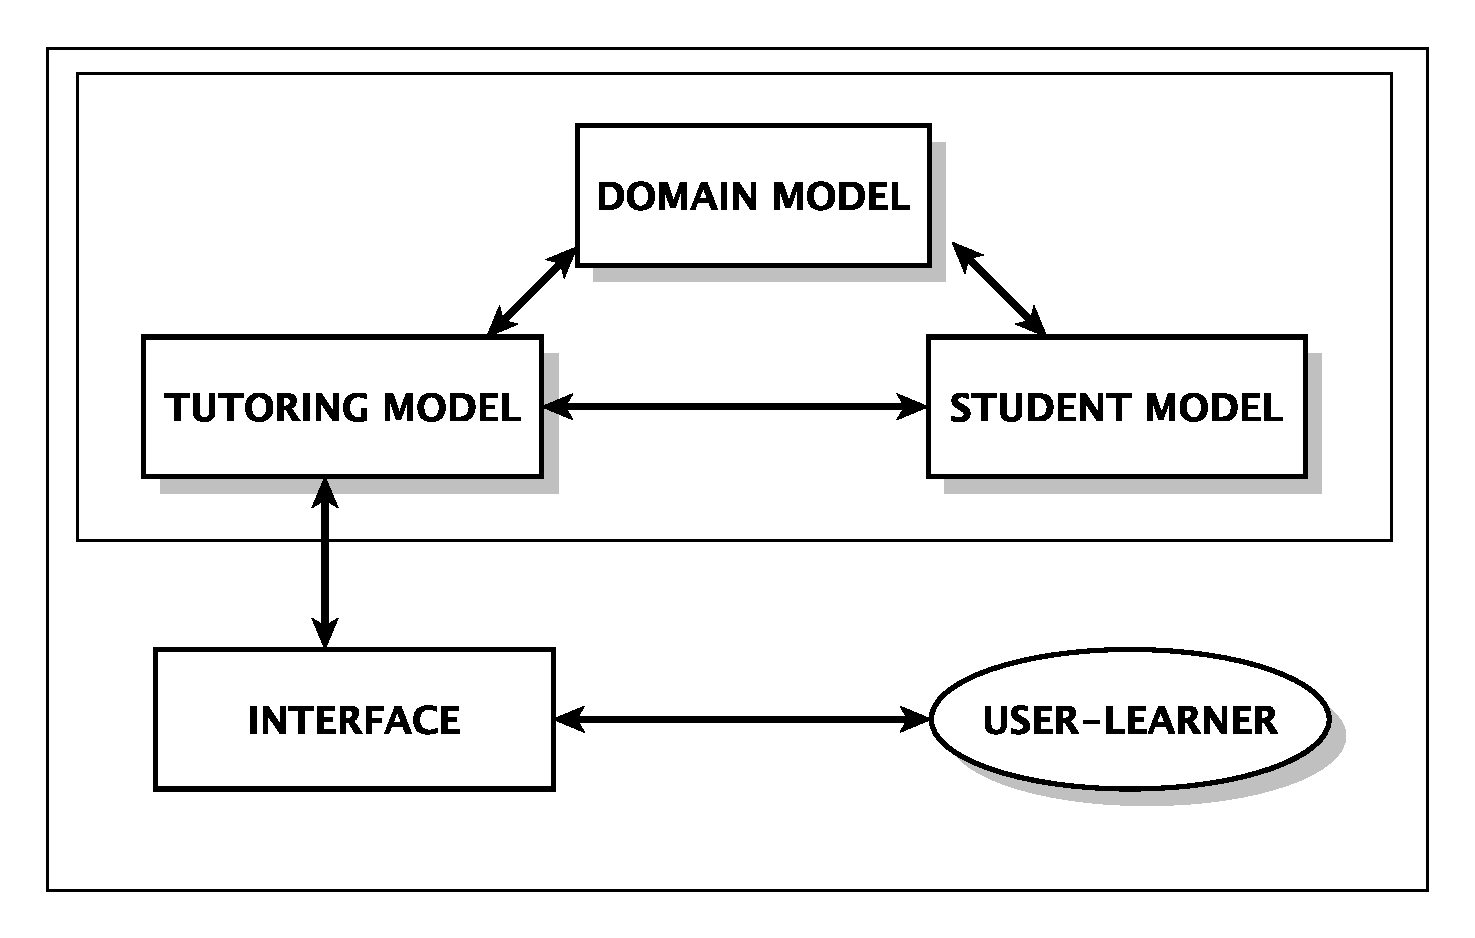
\includegraphics[scale=.3]{images/ITS.eps}
	\caption{The architecture of an intelligent tutoring system with its four components: the domain model, the student model, the tutoring model, and the user interface (taken from \cite{nkambou2010advances}).}
	\label{fig:ITS}       
\end{figure}
%%%%%%%%%%%%%%%%%%%%%%%%%%%%%%%%%%%%%%%

Starting from the 1970s, an artificial intelligence (AI) approach was proposed to add smart decision-making capabilities and more flexible features to the learning environment \cite{carbonell1970ai}. 
According to Holland \cite{holland2000artificial}, the history of AI in education
can be subdivided into a ``classical'' (from 1970 to 1987) and a ``modern'' (from 1987 to present days) phases. The ``classical'' phase focuses on the four elements of an intelligent tutoring system: the domain model, the student model, the tutoring model, and the user interface, as depicted in Figure~\ref{fig:ITS}. The domain model represents the expert knowledge and contains information about the domain to be taught. The student model should provide information about the student's level and progress. The tutoring model is fed by both the domain and the student model and is responsible for tutoring plans and content delivery. All this information flows through the interface which gives access to domain knowledge \cite{nkambou2010advances}. 

The ``modern'' phase extends AI features to embrace creativity and exploration, well beyond the simple assessment of already consolidated knowledge. Based on the Logo language introduced by Seymour Papert and his research team at MIT in  1967,\footnote{\url{https://el.media.mit.edu/logo-foundation/index.html}} this teaching philosophy produced ``MicroWorlds'', a multimedia learning environment aimed at involving students in more engaging learning activities and element manipulation. Originally conceived for learning mathematics \cite{edwards1995design}, the Logo system has been applied to music creation environments such as the ``Music Logo System'' \cite{bamberger1979} and ``LOCO'' \cite{desain1988}. Further approaches leverage on machine learning to make the students' experience richer and more personalized \cite{delgado2013learning}. Machine learning is used to support music performance software such as SmartMusic\footnote{\url{https://www.smartmusic.com/}} or music composition platforms such as Amper\footnote{\url{https://www.ampermusic.com/}} and Magenta.\footnote{\url{https://magenta.tensorflow.org/}}


%%%%%%%%%%%%%%%%%%%%%%%%%%%%%%

\section{Learning Theories}
\label{sec:theoryback}

During the last century, psychologists and researchers developed different theories on learning. The knowledge of the mechanisms through which the human brain learns is fundamental both for understanding the functioning of the various applications dedicated to music education and for their evaluation. It is also essential to acquire a historical perspective of the various theories in order to better understand future developments in this important domain. 

%%%%%%%%%%%%%%%%%%%%%%%%%%%%%%%%%%%%%%%%%%
\begin{figure}[t]
	\centering
	%\sidecaption
	\includegraphics[width=\columnwidth]{images/LT_CHART.png}
	\caption{Chart of the three reviewed learning theories with a short summary of learning definitions, historical contributions, instructional implications and examples of computer music applications. Freely adapted from Shunk~\cite{dale1991learning}.}
	\label{fig:LT}       
\end{figure}
%%%%%%%%%%%%%%%%%%%%%%%%%%%%%%%%%%%%%%%

A summary of the most important learning theories, mainly adapted from Shunk~\cite{dale1991learning}, is illustrated in Figure \ref{fig:LT}. The theories of behaviorism, cognitivism and constructivism are the most relevant in the field of computer-mediated education since they have specific areas of reference in the history of algorithms and computer systems. In the last row of Figure \ref{fig:LT}, these approaches have been exemplified in the form of music-oriented educational applications. The next subsections will cover in detail each of the three theories.

\subsection{Behaviorism}
\label{subsec:beh}
The origins of \textit{behaviorism} date back to Thorndike's theory of \textit{connectionism}, which considers learning as a series of associations between sensory experiences and neural impulses that manifest themselves through behaviors \cite{thorndike1913}. Thorndike's work was subsequently revised by Skinner, who in 1938 published his theory of \textit{operant conditioning} \cite{skinner1990behavior}. According to this theory, learners make associations between a given behavior and its consequences, favoring actions followed by pleasant effects compared to those followed by unpleasant ones. This mechanism leads to a reinforcement effect for the most repeated behaviors. 

The principles of operant conditioning have also been rendered by Skinner in \textit{programmed instruction} (PI) \cite{skinner1958teaching}, a series of instructional materials used to feed customized teaching machines. The material, organized in subsequent frames, is presented to learners with the request of a response. If correct, the machine moves to the next frame; if incorrect, a new similar frame is proposed with the aim of remedying the error. PI is organized in linear programs and branching programs, depending on how mistakes are treated. Linear programs proceed from frame to frame independent of the answer's accuracy; branching programs organize the sequence of frames according to the learner's answers, allowing to skip or to repeat frames depending on her/his ability. 

PI well represents typical behaviorist concepts, e.g.\ \textit{drill and practice}, which rely on repetition for the acquisition of new skills and on the adoption of rewards for \textit{positive} or \textit{negative} reinforcement. However, such an approach has often been judged as rigid and insufficiently compliant to adaptation \cite{mcdonald2005learning}. 

The previously discussed GUIDO system (1974)~\cite{hofstetter1975guido,eddins1981brief} provides an outstanding early example in music education, although for today's standards it offers limited flexibility and customization to learners' individual needs.


\subsection{Social Cognitivism}
In the early 1960s, behaviorism began to be challenged by many scholars and by different theories. One of these is Bandura's \textit{social cognitive theory} \cite{bandura1986social}, which relies on the observation that people can learn actions, gestures, skills and strategies by simply observing others in a social environment. Thus, learning may occur either by imitating models and evaluating the consequences of these modeled behaviors (\textit{enactive learning}) or by observing models performed in a live scenario or through symbolic or portrayed representations (\textit{vicarious learning}). 

Within this framework, important instructional implications may be outlined, such as \textit{teacher/peer modeling} and \textit{self-efficacy}. Teacher and peer models are a primary source of information as they can best guarantee for students' self-efficacy, that is the learner's ability of evaluating how well a given task can be executed. For this kind of learning, the availability of \textit{worked examples}, i.e., step-by-step demonstrations of how to accomplish a task, is crucial. Worked examples can be realized using visual and auditory texts and diagrams \cite{kalyuga2000incorporating} and are especially useful to reduce cognitive load and to ensure efficiency in delivering training materials. 

Other important teaching implications of cognitivism are \textit{tutoring} and \textit{mentoring} activities. \textit{Tutors} serve as instructional models for trainees, while \textit{mentors} extend advising and training activities to mutual learning and engagement between mentor and trainee. 

An early application of these theories to music education is ``The Piano Tutor'' by R.\ Dannenberg \cite{dannenberg1990computer}, a computer system which accompanies a beginner in the study of piano through the delivery of customized information and the processing of the student's input.

\subsection{Constructivism}

Strictly speaking, \textit{constructivism} is not a theory but, rather, a philosophical construct about the nature of learning  \cite{hyslop2007constructivism}. Constructivism rejects theoretical assumptions to be verified and tested, but supports the idea that learners themselves are the creators of their own knowledge~\cite{geary1995reflections}. 

The first contribution to constructivism comes from Piaget's theory of \textit{cognitive development}, which establishes that learning happens in a fixed sequence of stages: sensorimotor, preoperational, concrete operational and formal operational. Each stage defines how children interact with the world, thus acquiring the information necessary to make sense of their environment \cite{piaget1952origins}. 

Another important contribution to constructivism can be found in Vygotsky's sociocultural theory that emphasizes the social environment as a facilitator of development and learning. His \textit{Zone of Proximal Development} (ZPD) theory well describes the dynamic relationship between student and teacher. The student's task must be neither too simple to be accomplished alone nor too difficult to require the constant presence of the teacher. The ZPD is optimal when the teacher can provide only a final hint necessary to allow the student to accomplish the task \cite{vygotsky1980mind}. Another aspect of Vygotsky'work is \textit{activity theory}, which explains how learning happens through the interaction of a \textit{subject}, namely the learner, with an \textit{object} to be learned, mediated by a \textit{tool} supplied by the teacher and by a \textit{collaborative environment} 
\cite{jonassen1999activity}.

Constructivism has very important instructional implications, which engage teachers and learners in increasingly dynamic and stimulating relationships. \textit{Discovery learning} is one of these. The process of discovery involves making and testing hypotheses and using inductive reasoning to extend the study of single examples to general rules and concepts \cite{bruner1961act}. Learning through playing may also be considered as a part of discovery learning, as it involves some fundamental tenets of constructivism such as cognitive dissonance, application of new knowledge with feedback, and reflection on learning~\cite{baviskar2009essential}. Serious games are along these lines~\cite{barate2013serious}.

\textit{Inquiry teaching} -- a form of discovery learning -- is based on the Socratic teaching method, which consists in making questions and in stimulating answers aimed at augmenting critical thinking \cite{stevens2013cognitive}. \textit{Peer-assisted learning} in the forms of \textit{peer tutoring} and \textit{cooperative learning} greatly contributes to constructivism, providing cooperation among students and participation in achieving tasks that are too complex for individual learners. 

Another instructional implication of constructivism is \textit{reflective teaching}, which engages teachers in a continuous critical process of their actions, strategies, student motivation, and results. Being aware of context using personal and professional knowledge, making fluid plans, and carrying actions aimed at professional growth are the main characteristics of the reflective teacher \cite{savage2006teaching}. 

Constructivism, with the richness and variety of its theoretical background, represents the most popular framework in the design of instructional computer applications. An example is the already mentioned ``MicroWorlds'' by Seymour Papert \cite{papert1999logo}. The Logo language upon which ``MicroWorlds'' is based allows the design of highly interactive multimedia learning environments endowed with an on-screen pedagogical agent. ``MicroWorlds'' can be used for various purposes, including the study of computer programming \cite{mcnerney2004turtles}, mathematics \cite{hoyles1992pedagogy}, or technical subjects \cite{mayer2003multimedia}. 


%%%%%%%%%%%%%%%%%%%%%%%%%%%%%%

\section{Technology-Based Learning Approaches}
\label{sec:lrnappr}

The great number of tools and technologies available for teaching can create very rich and varied learning contexts and environments. Teaching today is not only a matter of organizing materials for frontal lessons in a classroom but, thanks to technology, of experimenting many other educational approaches. For instance, many computer applications allow music creation in an easy and intuitive way from the very early years \cite{farbood2004hyperscore, jennings2007composing, mcdowall2003music}. Their use requires the teacher to organize exploration activities and implies collaborative learning and experience sharing, a much richer and differentiated approach with respect to the traditional frontal lesson. 
New network technologies and the availability of portable devices make learning happen in many places, also outside schools and other formal contexts. This challenges teachers in revising their strategies and in introducing innovation in their practice \cite{de2014learning}. 

The present section focuses on the most relevant changes in the relationship between students and teachers and between students and knowledge related to the use of technologies. The aim is to outline the main learning situations that a student may face in a technological environment. Pedagogical aspects and implications are presented and analyzed starting from one of the main outcomes in the use of technologies, that is the ever-increasing coexistence of formal and informal learning in students' experience (Section \ref{subsec:FIL}). Aspects of online learning theories as well as the cultural landscape resulting from a constantly changing information stream are described in Section \ref{subsec:OL}. Section \ref{subsec:BL} is dedicated to blended learning, a teaching approach where the use of online or other computer technologies is mixed with the traditional face-to-face lesson modality. 
All these different approaches draw a composite picture where technology opens the way to a multidimensional character of music teaching and learning. 

\subsection{Formal and Informal Learning} \label{subsec:FIL}
Formal and informal learning are defined by Cross \cite[p. 12]{cross2011informal} not as dichotomies but rather as \textit{``[\ldots] ranges along a continuum of learning''}, as most learning experiences are a blend of both aspects. Distinguishing characteristics are outlined in Table \ref{tab:FIL}. 

%%%%%%%%%
\begin{table}[tb]
	\caption{Characteristics of Formal and Informal Learning. Adapted from 
		Cross~\cite{cross2011informal}.}
	\label{tab:FIL}  
	\centering     
	\begin{tabular}{p{0.45\columnwidth}p{0.45\columnwidth}}
		\hline\noalign{\smallskip}
		\textit{Formal Learning} & \textit{Informal Learning}  \\
		\noalign{\smallskip}\noalign{\smallskip}
		Is accomplished in school, courses, workshops, etc.. & Can happen everywhere\\
		Is scheduled in advance & Is not programmed and can happen both intentionally and inadvertently\\
		Realizes a curriculum & Considers learning as an open ended activity\\
		Requires that learners are evaluated and graded & Assigns no grade, since success in life is the measure of effectiveness\\
		\noalign{\smallskip}\hline\noalign{\smallskip}
	\end{tabular}
\end{table}
%%%%%%%%%

According to Folkestad ~\cite{folkestad2006formal}, in formal music learning, activities are scheduled in advance and their sequence is defined by the teacher, while, in informal music learning, the activity is steered by events (social interactions, creative processes, accidental discoveries) that occur during the experience.
Four ways of defining formal or informal music learning are identified: 

\begin{enumerate}
	\item \textit{situation}, i.e.\ the physical context (e.g., in the classroom or outside the school);
	\item \textit{learning style} (e.g.\ playing by written music or by ear);
	\item \textit{ownership}, i.e.\ who decides what to learn and where (e.g., didactic teaching or self-regulated learning);
	\item \textit{intentionality}, i.e.\ the aims towards which the mind is directed (e.g., learning how to play an instrument or just playing it).
\end{enumerate}

All these elements must be regarded in a dynamic way. For example, formal learning does not necessarily happen only inside the classroom, and informal learning only outside schools, as learning depends on intentionality, which is independent of the location. Formal learning is not even tied to determined music genres (e.g., classical music learned through music sheets), nor does informal learning apply exclusively to popular music learned by ear. Finally, Folkestad~\cite{folkestad2006formal} observes that learning can be formal or informal, but teaching is always formal by its nature. However teachers can embed in their programs situations where informal learning can happen (e.g., discussions) and can help transforming their pedagogical framing according to student progress.


\subsection{Online Learning}
\label{subsec:OL}
In the early 2000's, the WWW began to evolve from a ``read-only'' (Web 1.0) to a ``read-write'' modality (Web 2.0)~\cite{salavuo2008social}. This process -- popularized by Tim O'Reilly~\cite{oreilly} -- provides users not only with the ability to acquire information but also with the possibility to upload their own content and interact in real time with other users.  

Online learning environments are learning management systems that employ various methods and functionalities to deliver course materials: e-mails, notice boards, newsgroups, course outlines, conferences, multimedia repositories, and so on \cite{britain2004framework}.
Since the beginning, the main concern of designers was to avoid the mere reproduction of traditional teacher-centered class features, but rather to \textit{``[\ldots] use the powers of the computer to actually do better than what normally occurs in the face to face class.''} \cite[p. 1]{turoff1995}. Online learning environments build communities where students can shape and share their knowledge through autonomous investigations and peer-to-peer learning.  
Collaborative workspaces suggest a shift from the dominant learning model -- where the teacher transmits to learners an already consolidated wealth of information -- to a constructivist learning paradigm where learners are the architects of their own knowledge~\cite{jonassen1995constructivism}. 

Collaborative music making, music sharing, online music education, music games and widespread informal music learning are the new horizons opened by Web 2.0 applications~\cite{ruismaki2009new}. Keast~\cite{keast2009constructivist} suggests some guidelines for teaching music theory, history, and appreciation through online courses based on a constructivist approach. These include the availability of online materials (scores, audio and video) to allow students to investigate the topics independently, as well as tools for collaboration and self-assessment.  

An early example of collaborative music making is provided by Seddon~\cite{seddon2006collaborative}, who describes a shared composition experience between pairs of 13/14-year-old students belonging to Norwegian and English schools. Collaboration was asynchronously established through e-mails with textual and music exchanges. 
Collaborative music creation can also happen through creative interactions between multi-age students and web platforms for generative music making. In the work by Dillon et al.~\cite{dillon2009communities}, the platform displays a virtual music ensemble which allows direct manipulation of musical parameters and supports a sense of relationship and identity through the common music experience. These elements also characterize the many online music communities that have proliferated by exploiting existing social platforms (such as MySpace,\footnote{\url{https://myspace.com/}}  Facebook\footnote{\url{https://www.facebook.com/}} or MeetUp\footnote{\url{http://www.meetup.com/}})~\cite{salavuo2008social}. The main activities supported by online music communities include uploading one's music and expecting feedback, listening to contributed music and providing feedback, discussing and recommending music, connecting with other musicians in joint projects. 
%
A similar phenomenon is represented by the growth of online \textit{communities of practice}~\cite{waldron2009exploring,wenger1999communities}, which assemble groups of amateurs with shared interests on specific music genres.\footnote{An example about old-time American music styles is the Blue Ridge web site: \url{https://www.blueridgemusicnc.com/listen-and-learn/music-styles/old-time}.}


Communities of practice and social networking platforms share the same key working principles: participation, presence, and ownership. Salavuo~\cite{salavuo2008social} claims that the same key ideas should also support the design of online music education platforms, which should abandon models where a consolidated knowledge is distributed by an instructor in favor of a learner-centered education.

An important effect of online music learning is the diversification of music education environments, which are no longer restricted to classical music but can be extended in an easy and effective way to other genres. This enhances the promotion of cultural diversity and the openness towards cultural minorities~\cite{ruthmann2012music}. 



%%%%%%%%%%%%%%%%%%%%%%%%%%%%%%%%%%%%%%%%%%

\subsection{Blended Learning}
\label{subsec:BL}

According to Graham~\cite{graham2006blended}, blended learning systems \textit{``[\ldots] combine face-to-face instruction with computer-mediated instruction''}. Face-to-face environments have characterized the educational relationship for years, while the influence of computer-mediated instruction has been progressively growing in recent years. Face-to-face environments guarantee for a real, high-fidelity, human-to-human interaction, while computer-mediated instruction is distributed, self-paced, asynchronous, and puts emphasis on interactions between learners and materials. Under the pressure of communication technologies, the boundaries between these two approaches are rapidly thinning. Computer-supported collaboration, virtual communities and instant messaging provide an additional degree of humanness to computer learning environments, thus partially replacing the traditional functions of the teacher. 

The blended learning approach may include the following activities~\cite{louise2016impact}:
\begin{itemize}
	\item the use of electronic devices in the classroom (laptops, smartphones, tablets);
	\item the creation and use of online communities for sharing ideas, activities and materials;
	\item a synergy between computer and online resources and classroom activities;
	\item real-time posting of classroom discussions and activity materials;
	\item encouragement for students to share resources.
\end{itemize}

Blended learning does not only include a differentiation in the teaching activities but also implies a change in time and places where these activities occur. Watson~\cite{watson2008blended} defines blended learning as a shifting segment along a continuum which starts from a face-to-face setting with few or no online and technological resources available (the traditional classroom) and arrives to a fully online curriculum with all learning done outside the classroom and with no face-to-face component. In between,  various degrees of integration lay from traditional face-to-face to fully online instruction. Action places shift from the classroom through computer lab to everywhere; learning moments shift from the curricular lesson times through selected days in classroom and in lab to every time. 

The main feature of blended learning is students' control over 4 elements~\cite{roadmap}:
\begin{enumerate}
	\item \textit{Time} -- Learning is not restricted to school days but can happen anytime.
	\item \textit{Place} -- No need of classroom or school laboratory. Mobile devices and the ubiquity of internet allow access to learning materials from everywhere.
	\item \textit{Path} -- In the face-to-face modality the teacher decides the pedagogy and the approach to content. The free availability of learning materials can offer the self-tailored approach that better fits different students needs.
	\item \textit{Pace} -- Students can follow learning activities at their own pace without adapting to the learning rhythm of the entire class. 
\end{enumerate}

Online music learning environments can be also embedded within regular school programs~\cite{crawford2017rethinking}. Literature report case studies of group music composition in a blended learning environment~\cite{ruokonen2016learning} as well as the development of a participatory learning culture obtained by coupling face-to-face activities to an online discussion platform in a music technology class~\cite{draper2008hidden}.


%%%%%%%%%%%%%%%%%%%%%%%%%%%%%%

\section{Organizing Technology-mediated Music Knowledge}
\label{sec:OMTK}

In this section, we analyze frameworks and tools useful to organize the complex world of technology-mediated music knowledge. Firstly, we focus on the TPACK framework, where pedagogy, technology, and content information complement each other (Section~\ref{subsec:TPACK}). Secondly, we focus on the organization of knowledge in the musical domain and on the analysis of three artistic processes (Section~\ref{subsec:3AP}) which are important for classifying musical activities. In the light of these findings, new programs for the professional training of music teachers may be proposed. Furthermore, the organization of a music technology curriculum may benefit of both the TPACK framework and the mentioned standards. Finally, some approaches are presented and discussed in Section~\ref{subsubsec:MTC}.

\subsection{Technological Pedagogical and Content Knowledge (TPACK)}
\label{subsec:TPACK}

In his work, Shulman~\cite{shulman1986those} rejected the idea that teachers' knowledge is composed of two mutually exclusive fields, i.e., pedagogical knowledge and content knowledge. To cope with this dichotomy, he introduced the notion of ``Pedagogical Content Knowledge'' (PCK), which combines the two.
%According to Shulman, PCK corresponds to \textit{``[\ldots] the most useful forms of representation of the most powerful analogies, illustrations, examples, explanations, and demonstrations -- in a word, the ways of representing and formulating the subject [\ldots] that make it comprehensible to others''}. 
Building on Shulman's work, Mishra and Koehler~\cite{koehler2009technological} added the technological dimension to the framework, and proposed the ``Technological and Pedagogical Content Knowledge Paradigm'' (TPACK) specifically aimed at teaching and learning with technology. The resulting seven discrete types of knowledge are depicted in Figure~\ref{fig:TPACK}.

%%%%%%
\begin{figure}[t]
	\centering
	%\sidecaption
	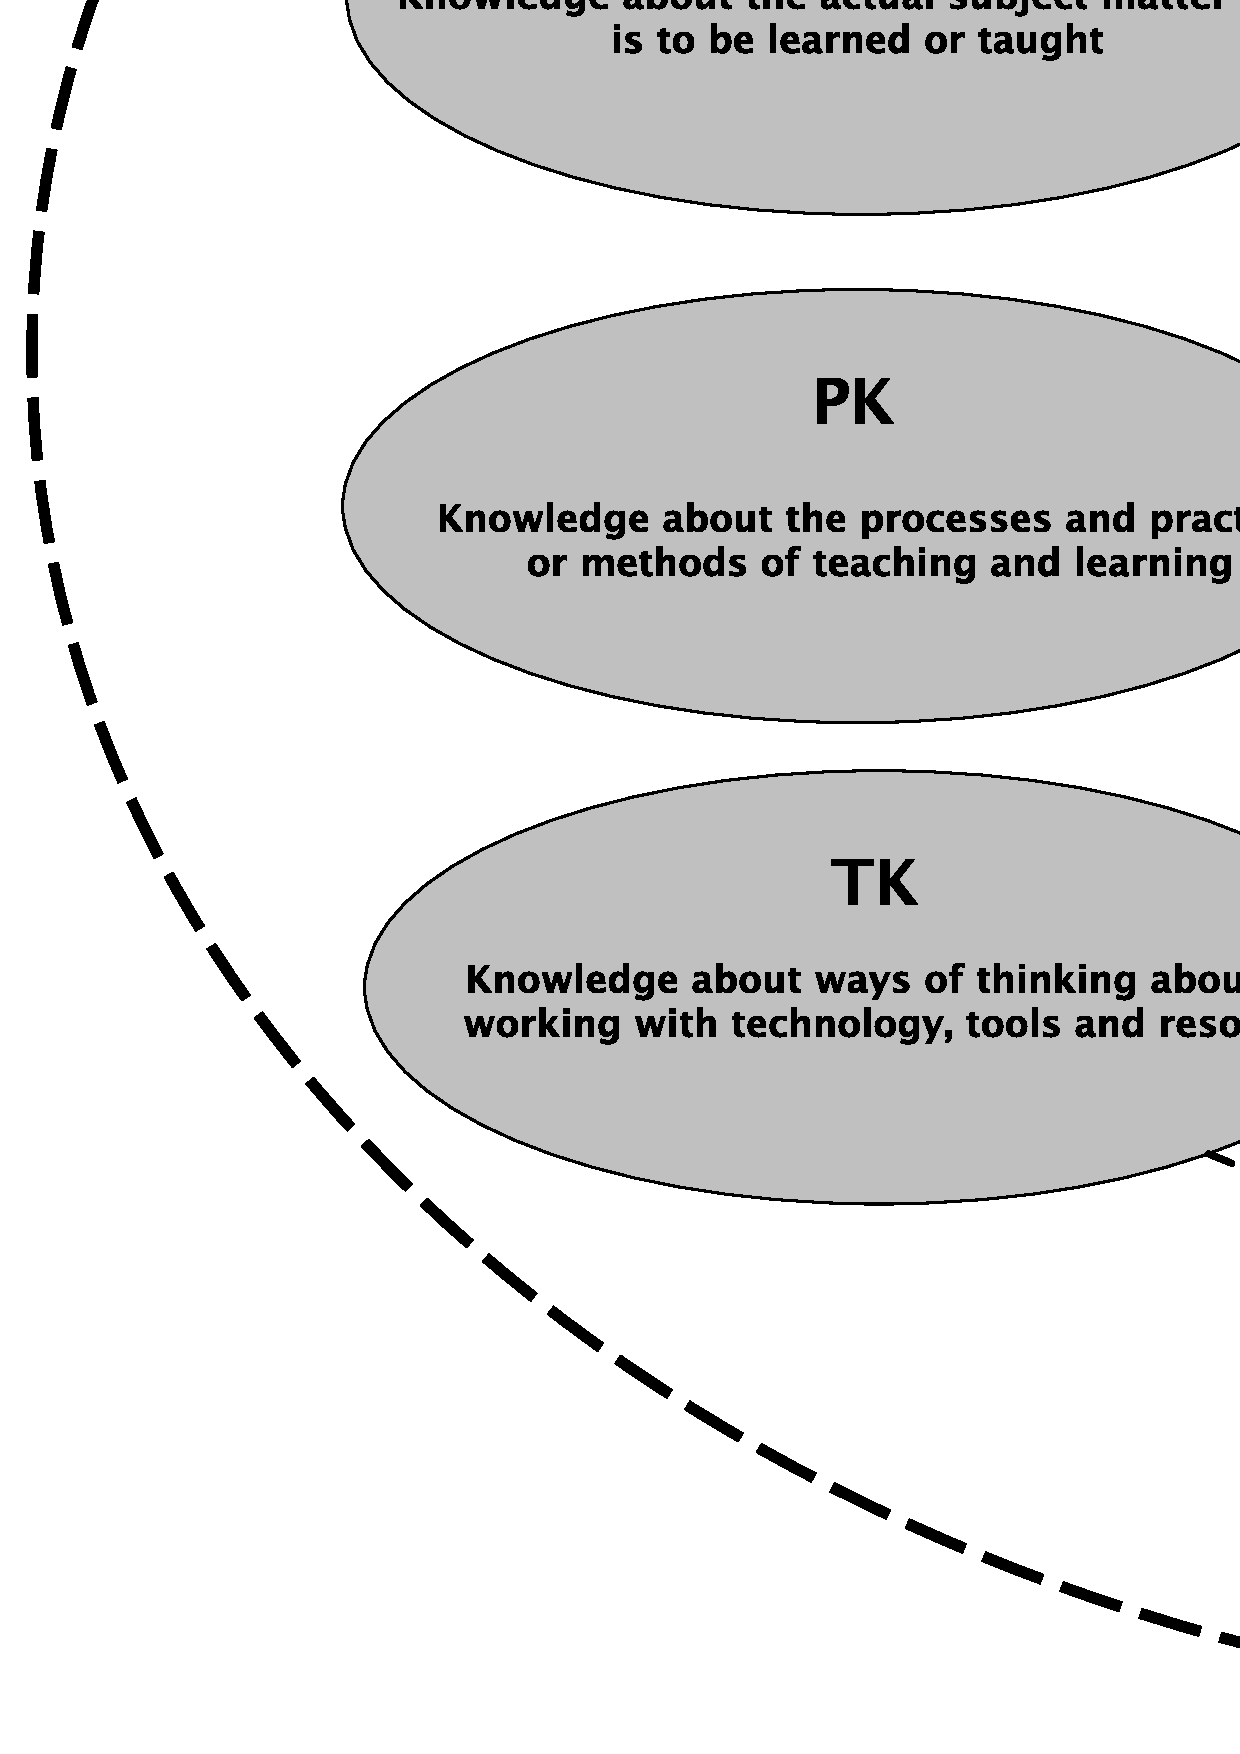
\includegraphics[width=\columnwidth]{images/TPACK.jpeg}
	\caption{Technological Pedagogical and Content Knowledge with the three forms of primary and secondary knowledge obtained by overlapping Content Knowledge, Pedagogical Knowledge and Technological Knowledge (adapted from the original http://www.tpack.org/).}
	\label{fig:TPACK}       
\end{figure}
%%%%%%

According to Bauer, when technology was introduced in schools it was a common belief that teachers would find by themselves the right ways to embed the potentials of the new tools in the curriculum of their students ~\cite{bauer2014music}. But very soon this turned out not to be true. Using technology effectively requires not only understanding technological means and how they work, but also being able to see and to interpret the dynamic relationships between technology, content, and pedagogical knowledge. These are summarized in Figure~\ref{fig:TPACK}, where the contents of the three primary forms of knowledge (CK, PK, and TK) are paired to generate three new secondary forms (PCK, TCK and TPK).
TPACK is the result of the overlapping of all the three forms. 
The ``contexts'' label surrounds the diagram to indicate the situated nature of TPACK. This means that TPACK is a flexible framework compliant to physical constraints (classroom, laboratory, technological equipment available) as well as to cultural constraints (class level, course aims, students' attitudes, and so on). 


TPACK outlines a rich and varied knowledge structure for teachers to profitably use technology in their work. This raises the question of how to design a curriculum for these teachers.
As Koehler and Mishra point out~\cite{koehler2005happens}, embedding music technology workshops in pre-service music educators curricula is not enough to train teachers who will be aware and able to apply technology in their educational practices~\cite{brand1998research, duran2006technology, haning2016they}. 
Teaching technology by design is the best way to make TPACK effective. However, this requires a high level of ability in managing the rich context provided by this factual approach~\cite{koehler2009technological}. By contrast, the reality reported by research in the field is that the main obstacle to the use of technology in schools is simply that teachers are not prepared to use it~\cite{dorfman2016exploring}. 

Authenticity of integration, lack of administrative, technological, and pedagogical support, limited access to technology and/or funding, lack of space in the curriculum, are reported among the main obstacles met by teachers~\cite{bakir2015exploration, bauer2016technology, dorfman2016music, eyles2018teachers}. However, teachers' competences in the use of digital materials remains the main impact factor for the integration of technology in the classroom~\cite{trainin2018impact, wise2011teachers} and, for this reason, music technology training programs in pre-service curricula are strongly recommended~\cite{bakir2015exploration}.


%%%%%%%%%%%%%%%%%%%%%%%%%%%%%%%%%%%%

\subsection{The National Standards for Music Education}
\label{subsec:3AP}
Developed by NCCAS (National Coalition for Core Arts Standards),\footnote{NCCAS is an alliance of national arts and arts education organizations who formed in 2011 and dedicated to the work of creating and supporting national arts standards (\url{https://sites.google.com/nccas.org/nccas-wikispace})} the last version of the National Core Arts Standards was released in 2014.\footnote{\url{https://www.nationalartsstandards.org/}} The aim of the standards is to identify the learning that each student must achieve in the artistic field, thus helping teachers in developing and organizing their own teaching programs. The standards derive from the observation of the artistic processes through which artists communicate with their audience and with the society around them. The standards are  cognitive and physical actions through which art is realized and, consequently, represent a reliable link between art making and the learner~\cite{NCCAS}. 

%%%%%%%%%
\begin{table*}[htbp]
	\caption{Artistic Processes Definitions and Standards, adapted from~\cite{NCCAS}.}
	\label{tab:AP}
	\centering
	\begin{tabular}{p{0.1\textwidth}p{0.3\textwidth}p{0.5\textwidth}}\\
		ARTISTIC & DEFINITIONS & STANDARDS\\
		PROCESSES & &\\
		\hline\noalign{\smallskip}
		Creating & Conceiving and developing new artistic ideas and work &1. Generate and conceptualize artistic ideas and work.\newline
		2. Organize and develop artistic ideas and work.\newline
		3. Refine and complete artistic work.\\
		\hline\noalign{\smallskip}
		Performing & Realizing artistic ideas and work through interpretation and presentation & 4. Select, analyze, and interpret artistic work for presentation.\newline
		5. Develop and refine artistic techniques and work for presentation.\newline
		6. Convey meaning through the presentation of artistic work.\\
		\hline\noalign{\smallskip}
		Responding & Understanding and evaluating how the arts convey meaning &
		7. Perceive and analyze artistic work.\newline
		8. Interpret intent and meaning in artistic work.\newline
		9. Apply criteria to evaluate artistic work.\\
		\hline\noalign{\smallskip}
	\end{tabular}
\end{table*}
%%%%%%%%%

The 9 standards outlined in Table \ref{tab:AP} are grouped in the 3 broad areas of artistic processes (``Creating'', ``Performing'' and ``Responding''). While NCCAS includes a fourth area (``Connecting''), for music this is considered to be embedded in the three previous areas~\cite{NAfme}.

According to Shuler~\cite{shuler2011music}, artistic processes are also compliant with the so-called \textit{four Cs} model. The four \textit{Cs} refer to:
\begin{itemize}
	\item \textit{Creativity} -- The standards support creativity by suggesting the students to engage in improvisation, composition and interpretation of music;
	\item \textit{Critical thinking} -- The standards support critical thinking by suggesting the students to select music pieces, to refine performances and compositions and to interpret intent and meaning of music;
	\item \textit{Communication} -- This is the primary purpose of the arts. Students learn to communicate while performing or composing music, or while expressing their musical ideas during the ``Responding'' process;
	\item \textit{Collaboration} -- This skill resides upon teachers' ability in fostering group decisions through student-directed sectionals, chamber ensembles and collaborative composition groups.
	
\end{itemize}

Although released for the United States, most standards for arts education in other countries seem to build on the same three areas \cite{AC, AEKLA, NCE, PSC}. Thus, the framework of ``Creating'', ``Performing'' and ``Responding'' may be considered as a sound and widely shared system for organizing artistic knowledge and educational activities.

\subsection{Embedding Technology in Music Curricula}
\label{subsubsec:MTC}

%%%%%%%%%
\begin{table*}[htbp]
	\caption{Some ideas for connecting technology to the 1994 music standards, adapted from %Rudolph (2004) 
		\cite{rudolph2004teaching}.}
	\label{tab:rudolph}
	\centering
	\begin{tabular}{p{0.3\textwidth}p{0.3\textwidth}p{0.3\textwidth}}\\
		STANDARDS (1994) & DEVICES \& SOFTWARE & ACTIVITIES\\
		\hline\noalign{\smallskip}
		1. Singing, alone and with others, a varied repertoire of music & MIDI keyboard and sequencing software & Create, record and playback accompaniments\\
		& Claire and Audio Mirror software & Analyze the singing voice and receive feedback to improve performance
		\\
		\hline\noalign{\smallskip}
		2. Performing on instruments, alone and with others, a varied
		repertoire of music & Electronic keyboards & Play bands or various ensembles replacing missing instruments\\
		
		\hline\noalign{\smallskip}
		3. Improvising melodies, harmonies, and accompaniments & MIDI keyboard and sequencing software & Play accompaniments while exploring improvisation \\
		& Band-in-a-Box & Experiment with harmonies and accompaniments\\
		\hline\noalign{\smallskip}
		
		4. Composing and arranging music within specified guidelines & Notation software & Compose and listen\\
		
		\hline\noalign{\smallskip}
		5. Reading and notating music & Notation software & Create printed scores
		\\& Computer-assisted instruction software & Recognize rhythm and tonal patterns\\
		
		\hline\noalign{\smallskip}
		6. Listening to, analyzing, and describing music & Computer-assisted instruction software & Learn music theory and ear training\\
		
		\hline\noalign{\smallskip}
		7. Evaluating music and music performances & MIDI keyboard and sequencing software & Playback of music pieces\\

		& MIDI keyboard and notation software & Compare performances with the printed score\\
		
		\hline\noalign{\smallskip}
		8. Understanding relationships between music, the other arts,
		and disciplines outside the arts & Electronic keyboards and multimedia software & Create and modify sounds, linking music with science and mathematics\\
		
		\hline\noalign{\smallskip}
		9. Understanding music in relation to history and culture & CD-ROM & Listen to music with text, images and videos\\
	\end{tabular}
\end{table*}
%%%%%%%%%

According to Rudolph~\cite{rudolph2004teaching}, the simplest way to build a music curriculum based on technology is to use computers and electronic devices to enhance the 9 music standards. To this end, he combines the potentialities of available technologies with the 1994 music standards, as outlined in Table \ref{tab:rudolph}. The result is an effective and consistent operational framework. Even if the considered equipment is limited and outdated with respect to present days, the connections between standards, technologies, and activities are sound and clearly show the new possibilities offered by electronic devices and software. 

A complementary approach is followed by Watson~\cite{watson2011using}, who starts from available technologies to propose a series of lesson plans aimed at enhancing students' creativity. The range of available devices and software comprises:
\begin{itemize}
	\item electronic keyboards;
	\item sound recording applications;
	\item multi-track music production applications;
	\item computer music notation applications;
	\item instructional software and other music applications.
\end{itemize}

Lesson plans are built upon a set of principles aimed at facilitating students' creativity.
For each lesson plan, the corresponding national standards addressed are outlined as a reference framework for the various proposed activities.

The work of Bauer~\cite{bauer2014music} is particularly relevant because it builds on the three artistic processes of ``Creating'', ``Performing'' and ``Responding'' in order to build a taxonomy of music activity types. Despite the fact that in every music activity these three processes are inextricably present at various degrees, Bauer et al. 
%(2012) 
\cite{bauerharris} make an analytical effort to group activity types in each of the three areas, including technological facilities such as software, applications and other instructional material. Bauer's taxonomy is summarized in Table \ref{tab:bauer}.
%%%%%%%%%%
%%%%%%%%%
\begin{table*}[htbp]
	\caption{The taxonomy of music activities adapted from Bauer~\cite{bauerharris, bauer2014music}.}
	\label{tab:bauer}
	\centering
	\begin{tabular}{p{0.2\textwidth}p{0.2\textwidth}p{0.5\textwidth}}
		ARTISTIC  & MUSIC & ACTIVITY \\
		PROCESSES  & ACTIVITIES & TYPES \\
		\hline\noalign{\smallskip}
		CREATING & Improvisation & 1. Echo rhythm and tonal patterns\\
		& (a) & 2. Improvise a tonal or rhythmic answer to a tonal/rhythmic prompt\\
		& & 3. Perform familiar melodies and/or their bass lines by ear\\
		& & 4. Improvise rhythmic and/or melodic variations on a familiar melody\\
		& & 5. Perform melodic patterns in a variety of keys/tonalities\\
		& & 6. Improvise an original melody to a given accompaniment\\
		& & 7. Transcribe a solo\\
		& & 8. Improvise in a group\\
		& & 9. Improvise an accompaniment\\
		& & 10. Engage in free improvisation\\
		
		\cline{2-3}
		
		& Composition & 1. Create an ostinato\\
		& (b) & 2. Use non traditional sounds to create music prompt\\
		& & 3. Create or utilize an alternative notation\\
		& & 4. Compose an ``answer'' phrase to a given ``question'' phrase\\
		& & 5. Compose a melodic variation\\
		& & 6. Compose using repetition and contrast\\
		
		& & 7. Create a loop-based composition\\
		& & 8. Create a remix\\
		& & 9. Arrange music\\
		& & 10. Compose an accompaniment\\
		& & 11. Create a composition\\
		& & 12. Compose a video soundtrack\\
		%%%performing
		\hline\noalign{\smallskip}
		PERFORMING & Singing (c)& 1. Sing with a steady beat\\
		& & 2. Sing with appropriate posture, breath support, and diction\\
		& & 3. Sing individually\\
		& & 4. Sing in an ensemble\\
		& & 5. Sing with technical accuracy\\
		& & 6. Sing with expression\\
		& & 7. Listen to/view vocal/choral models\\
		& & 8. Respond to the gestures of a conductor when singing\\
		& & 9. Cover a song\\
		
		\cline{2-3}
		
		& Playing (d)& 1. Play with a steady beat\\
		& & 2. Play with appropriate posture and technical (motor) skills\\
		& & 3. Play individually\\
		& & 4. Play in an ensemble\\
		& & 5. Play with technical accuracy\\
		& & 6. Play with expression\\
		
		& & 7. Listen to/view instrumental models\\
		& & 8. Respond to the gestures of a conductor when playing\\
		& & 9. Cover a song\\
		
		\cline{2-3}
		
		&  Reading & 1. Clap/sing with rhythm syllables, sing/play varying rhythm patterns\\
		& and notating & 2. Sing with solf\`{e}ge syllables, sing/play varying pitch patterns\\
		& music (e) & 3. Identify and interpret musical symbols\\
		&  & 4. Read standard notation while singing or playing\\
		
		&  & 5. Sight read accurately\\
		&  & 6. Aurally identify and/or notate patterns\\
		&  & 7. Notate music\\
		
		\hline\noalign{\smallskip}
		RESPONDING & Listening and & 1. Listen repeatedly\\
		& Describing (f)& 2. Listen to examples\\
		& & 3. Guided listening\\
		& & 4. Listen to, describe, and discuss music\\
		& & 5. Listen and reflect\\
		
		\cline{2-3}
		
		& Analyzing (g)& 1. Move in response to music\\
		& & 2. Identify and label structural and expressive components of music\\
		& & 3. Describe and discuss structural and expressive components of music\\
		& & 4. Develop an analysis\\
		& & 5. Develop an interpretation\\
		
		\cline{2-3}
		
		&  Evaluating (h)& 1. Develop criteria for evaluating a musical performance, improvisation, composition, or arrangement\\
		&  & 2. Critique a musical performance, improvisation, composition, or arrangement\\
		&  & 3. Provide constructive suggestions for improvement of a musical performance, improvisation, composition, or arrangement\\
		&  & 4. Create a musical portfolio\\
		\hline\noalign{\smallskip}
	\end{tabular}
\end{table*}


%%%%%%%%%%%%%%%%%%%%%%%%%%%%%%

\section{A Multidimensional Taxonomy of Digital Learning Materials}
\label{sec:MTDLM}

Bauer's taxonomy   
offers a detailed and comprehensive view of the activity types that can compose a music curriculum. For this reason, this taxonomy will be used as the main reference for classifying musical activities enabled by technology. 
%
On the other hand, musical activities are not enough for classifying digital learning materials. As emphasized by the TPACK framework (Section \ref{subsec:TPACK}), the content domain (i.e., artistic processes) need to be integrated with the pedagogical and technological domains. This widens substantially the perspective on digital materials for music education, and makes them a much complex and multifaceted knowledge field. 

An useful tool for properly representing this level of complexity is provided by  \textit{multidimensional taxonomies}. According to Law et al. \cite{law1998toward}, a multidimensional taxonomy consists of a number of associated dimensions belonging to different domains. By applying this definition to the field of digital materials for music education, we elaborated a multidimensional construct organized in three levels. The first level includes \domain{Metadata} and the three \domain{Technological}, \domain{Musical}, and \domain{Pedagogical} domains corresponding to the TPACK framework. The second level holds an overall number of 10 dimensions, 3 for \domain{Metadata} and 7 for the \domain{Technological}, \domain{Musical}, and \domain{Pedagogical} domains. The third level deploys all the nodes derived from the analysis of the database in each dimension.

The proposed taxonomy is summarized in Table~\ref{tab:tax}.
In this section we describe the research steps that led us first to the creation of a database of scientific contributions related to music education applications (Section~\ref{subsec:resm}) and then to the creation of the taxonomy, whose domains are analyzed in Sections~\ref{subsec:TD},~\ref{subsec:MD}, and~\ref{subsec:PD}, together with related application examples taken from the database. Finally, Section~\ref{subsec:exploring} presents a web interface for navigating the database and producing comparison charts between the taxonomy dimensions.

\begin{table*}[htbp]
	\caption{The 3 levels of the taxonomy with associated domains, dimensions, and nodes.}
	\label{tab:tax}
	\centering
	\begin{tabular}{p{0.25\textwidth}|p{0.25\textwidth}|p{0.4\textwidth}}
		\hline
		1\textsuperscript{st} LEVEL: \domain{Domains} &  2\textsuperscript{nd} LEVEL: \dimension{Dimensions} & 3\textsuperscript{rd} LEVEL: \node{Nodes}\\
		\hline
		& \dimension{0.0. Material} (resource) & \node{0.0.0. Name}\\
		\cline{2-3}
		& & \node{0.1.0. Evaluation}\\
		& & \node{0.1.1. Presentation}\\
		\domain{0. Metadata} & \dimension{0.1. Contribution} (type) & \node{0.1.2. Case study}\\
		& & \node{0.1.3. Review}\\
		& & \node{0.1.4. Practices}\\\cline{2-3}
		& \dimension{0.2. Date} (year) & \node{0.2.0 20xx}\\
		\hline
		& & \node{1.0.0. Desktop}\\
		& & \node{1.0.1. VR, AR}\\
		& \dimension{1.0. Application} (object) & \node{1.0.2. Tangible computing}\\
		& & \node{1.0.3. Mobile computing}\\
		& & \node{1.0.4. Smart rooms}\\
		\cline{2-3}
		& & \node{1.1.0. Mouse, keyboard}\\
		& & \node{1.1.1. MIDI}\\
		& & \node{1.1.2. Mobiles}\\
		\domain{1. Technological} & \dimension{1.1. Enabling Technologies} (input) & \node{1.1.3. Tangibles and wearables}\\
		& & \node{1.1.4. Camera}\\
		& & \node{1.1.5. Microphone}\\
		& & \node{1.1.6. Electric instruments}\\
		\cline{2-3}
		& & \node{1.2.0. Audio}\\
		& & \node{1.2.1. Visual}\\
		& \dimension{1.2. System Output} (output) & \node{1.2.2. Video}\\
		& & \node{1.2.3. Haptic}\\
		& & \node{1.2.4. Raw data}\\
		\hline
		& & \node{2.0.0. Creating}\\
		\domain{2. Musical} & \dimension{2.0. Activity} (aim) & \node{2.0.1. Performing}\\
		& & \node{2.0.2. Responding}\\
		\hline
		& & \node{3.0.0. Behaviorism}\\
		& \dimension{3.0. Learning Theories} (models) & \node{3.0.1. Cognitivism}\\
		& & \node{3.0.2. Constructivism}\\
		\cline{2-3}
		& & \node{3.1.0. Pre-school, primary}\\
		& & \node{3.1.1. Secondary}\\
		\domain{3. Pedagogical} & \dimension{3.1. Users} (recipients) & \node{3.1.2. Conservatory, university}\\
		& & \node{3.1.3. Adults M and NM}\\
		& & \node{3.1.4. Not defined}\\
		\cline{2-3}
		& & \node{3.2.0. Classroom}\\
		& \dimension{3.2. Venue} (place) & \node{3.2.1. Lab}\\
		& & \node{3.2.2. Everywhere}\\
		& & \node{3.2.3. Web}\\
		\hline
	\end{tabular}
\end{table*}
%%%%%%%%%%%%%%%%%%%%

\subsection{Research Methodology}
\label{subsec:resm}

We conducted an extensive research  in order to build a database containing scientific publications on digital materials aimed at music education. The choice to focus exclusively on scientific publications (journal articles, conference proceedings, books, book chapters and, only exceptionally, master's or doctoral theses) was dictated by the need to obtain the most reliable information on the digital materials, the use they are intended for, and the educational experiences connected to them. 

This approach, while providing information about end users and sometimes about application assessment in teaching contexts, excludes two important categories of materials. The first one embraces the many undocumented web sites that offer services, software, games, applications and platforms for music education for both computer and mobile devices; the second category includes commercial applications or services. Both these categories are difficult to study for several reasons. Freely usable web sites are designed for the most varied purposes, ranging from music resources repositories \cite{BBC, K12}, to ear training and music theory applications \cite{FET, MT} and web sites that support instrumental practice \cite{gstrings, PTG}. Although some of them have a clear connection to educational practices and actually constitute valid teaching and learning resources, the lack of documentation can make their categorization questionable or undetermined. Moreover, commercial applications use proprietary software whose characteristics -- for obvious reasons -- are not made public; usability data that would be needed for evaluating the efficiency of applications are not easily accessible too. All these aspects would require to adapt the analytical approach. For this reason, a thorough analysis of undocumented online resources and commercial applications is left for future work.



The research of scientific publications related to digital materials for music-education went through different phases. The first phase involved research using generic keywords such as ``music learning applications'', ``music education technology'' or ``computer aided music education''. This research was carried out both through the main search engines on the web and through databases dedicated to academic literature, such as ACM Digital Library,\footnote{\url{https://dlnext.acm.org/}} Google Scholar,\footnote{\url{https://scholar.google.com/}} CiteseerX,\footnote{\url{https://citeseerx.ist.psu.edu/}} IEEE Xplore Digital Library,\footnote{\url{https://ieeexplore.ieee.org/}} JSTOR,\footnote{\url{https://www.jstor.org/}} and Scopus.\footnote{\url{https://www.scopus.com/}} Secondly, after the collection of the first batch of papers, a bibliography-based search was carried out in the same way. Thirdly, at this point a list of the main journals devoted to music education digital materials emerged. Archives of specific journals (e.g., the British Journal of Educational Technology,\footnote{\url{https://onlinelibrary.wiley.com/journal/14678535}} the British Journal of Music Education,\footnote{\url{https://www.cambridge.org/core/journals/british-journal-of-music-education}} Computers \& Education,\footnote{\url{ttps://www.journals.elsevier.com/computers-and-education/}} International Journal of Educational Research,\footnote{\url{https://www.journals.elsevier.com/international-journal-of-educational-research/}} Journal of Music, Technology and Education,\footnote{\url{https://www.ingentaconnect.com/content/intellect/jmte}} Music Education Research,\footnote{\url{https://www.tandfonline.com/toc/cmue20/current}} etc.) were also examined. Finally, once the nodes of the taxonomy were defined, a search employing the keywords of those nodes was also carried out.



Exclusion criteria were applied on the retrieved academic papers. Contributions reporting music applications not explicitly aimed at education were discarded. A temporal filter was also applied to avoid obsolete systems and old applications. Thus, only papers written after year 2000 were kept in the database.
The collection of scientific papers is still in progress and currently amounts to a total of 124 entries.
%%%%%%%%%%
%%%%%%%%%%

\subsection{The Metadata Domain}
\label{subsec:MeD}

The \domain{Metadata} domain of the taxonomy includes the following 3 dimensions: 

\begin {enumerate}[label=0.\arabic*.,leftmargin=0.7cm,listparindent=-\leftmargin, start=0]

\item \dimension{Material} -- This dimension reports the name of the application, if explicitly indicated in the publication; in other case, we assign the application a self-explanatory name followed by the label ``(attr.)'' to emphasize that the name is not original. Currently, 137 applications have been gathered in the database;

\item \dimension{Contribution} -- This dimension indicates the type of research contained in the article. Concerning nodes, a scientific paper can be an \node{Evaluation} (description of the application and results of users tests), a \node{Presentation} (description of the application only), a \node{Case study}, a \node{Review} or \node{Practices} (teaching experiences or methods);

\item \dimension{Date} -- This dimension takes into account the year of publication. Only publications issued after 2000 have been included in the database.

\end{enumerate}

The distribution of items for the \dimension{Contribution} dimension is represented in the chart of Figure \ref{fig:0102}.

%%%%%%%%%%%%%%%%%%%%%%%%%%%%%%%%%%%%%%%%%%
\begin{figure}[t]
\centering
\includegraphics[height=2in]{images/01.pdf}  
\caption{Distribution of items for the ``0.1. Contribution'' dimension.}
\label{fig:0102}       
\end{figure}
%%%%%%%%%%%%%%%%%%%%%%%%%%%%%%%%%%%%%%%

\subsection{The Technological Domain}
\label{subsec:TD}

Concerning the \domain{Technological} domain, its dimensions refer to the technical aspects of the applications. In particular, we focus on human-computer interaction as the most meaningful technological aspect seen from the user's side. Karam \& Schraefel, in their taxonomy of users gestures in human-computer interaction, propose a classification based on 4 categories: application domains, enabling technologies, system response and gesture styles~\cite{karam2005taxonomy}. This framework allows a clear definition of the kind of application, of the technologies employed for data input and of the system output modalities. We rearranged the taxonomy on the basis of the characteristics of music-education digital materials. Specifically, the gesture-style category has been discarded in the present proposal because, differently from from Karam \& Schraefel, gestures are not the focus of our research. 

The \domain{Technological} domain then includes the following 3 dimensions:
\begin{enumerate}[label=1.\arabic*.,leftmargin=0.7cm,listparindent=-\leftmargin, start=0]

\item \dimension{Application} -- This dimension refers to the kind of digital artefact employed in the learning activity, i.e., the object of the action. The nodes of this dimension are:

\begin{enumerate}[label=1.0.\arabic*.,leftmargin=0.9cm,listparindent=-\leftmargin, start=0]

\item \node{Desktop} -- This is an umbrella term that includes all software running on a personal computer, including music sequencers, DAWs and audio editors (e.g. \textit{Audacity},\footnote{\url{https://www.audacityteam.org/}}) tutoring systems~\cite{schoonderwaldt2004imutus}, games~\cite{smith2009effect}, as well as programming environments (e.g., \textit{Pure Data} and \textit{Max/Msp});
%
\item \node{Virtual Reality (VR), Augmented Reality (AR)} -- These applications provide \textit{``[\ldots] a real or simulated environment in which a perceiver experiences telepresence''}, as in the case of VR~\cite[p. 7]{steuer1992defining}, or superimpose virtual objects in a real environment, as for AR~\cite{azuma1997survey}. Typical examples of AR in music education are the systems for learning how to play instruments through information projected on the keyboard for piano or on the fretboard for guitar \cite{lochtefeld2011guitar, rogers2014piano}; 
%
\item \node{Tangible computing} -- These applications include systems capable of receiving and processing data coming from the manipulation of physical objects or from wearable and touch sensors. One of the most famous systems in this dimension is the \textit{Reactable}, which can be used both for music creation and education \cite{franceschini2010towards, xambo2013let}, while a recent device based on tangibles is Kodaly Kibo \cite{al2020kiboa};
%
\item \node{Mobile computing} -- This node covers applications mainly designed for tablets and smartphones. Mobile computing is based on touch and pressure interaction and allows learning independent of traditional time and space constraints. Examples in this dimension are \textit{JamMo}, a software for children's mobile music making~\cite{paananen2009jammo} and the many apps for music activities for the iPad presente in~\cite{ruismaki2013ipad};
%
\item \node{Smart rooms} -- These are large-scale interactive environments that respond to user movements or gestures. The \textit{Sound Maker} \cite{antle2008playing} for music creation and \textit{Harmonic Walk} \cite{mandanici2016harmonic} for melody harmonization are good examples. Interaction in smart rooms is based on body awareness and skills such as proprioception and kinesthesia  \cite{jacob2008reality}. The effects of bodily interaction and the possibility of sharing the learning experience with bystanders have not been deeply studied yet, and it is not clear how these factors influence the learning process \cite{johnson2009smallab, zanolla2013entertaining}. 
\end{enumerate}

\item \dimension{Enabling technologies} is a dimension that groups all the technologies used for input of music data and of music performers' motion. The nodes in this dimension are:

\begin{enumerate}[label=1.1.\arabic*.,leftmargin=0.9cm,listparindent=-\leftmargin, start=0]

\item \node{Mouse and keyboard} -- These are the most traditional and widespread devices used for interacting with the computer, also in the musical domain. The mouse is the main pointing device to manipulate the graphical elements used in music production environments such as DAWs and sequencers, while the keyboard is used for quick note and duration input in score editors;
\item \node{MIDI} -- MIDI, an acronym for Musical Instrument Digital Interface, is a technical standard that describes a communications protocol, a digital interface, and the electrical connectors that let a wide variety of electronic musical instruments, computers, and other audio devices exchange data. In an educational context, the data produced by MIDI devices (mainly controllers such as electronic keyboards and pads) can be used to feed music notation software~\cite{schroth2009using}, sequencers~\cite{mcdowall2003music} and tutoring systems for computer assisted music performance~\cite{barakonyi2005augmented};
\item \node{Mobiles} -- Tablets and smartphones are used as wireless input devices for music education software in a variety of ways. They can act as distributed controllers of the audio events as in the \textit{Soundcool} project~\cite{berbel2017sound}; or can provide a surface for percussive performance as in the \textit{Rhythm Workers} application~\cite{begel2018rhythm}. They can also be used as image input tools for augmented reality music education applications~\cite{rusinol2018augmented} or -- through the inertial sensors of a smartphone -- as input devices to decide the virtual walk's direction as in the \textit{VR4EDU} application~\cite{degli2019mobile};
\item \node{Tangibles, wearables} -- Musical interaction of sensorized physical objects may happen through their creative manipulation~\cite{weinberg2002beatbug} and~\cite{bakker2010moso}) or by arranging them on a customized board~\cite{parra2014}. Wearables can be used to detect the motions of a violin player as in the \textit{MusicJacket}~\cite{johnson2010musicjacket} or to act as markers for a computer vision system devoted to pitch, rhythm and timbre detection~\cite{martins2015teaching};
\item \node{Camera} -- Cameras provide live video and motion data a music performance. Live videos can be used to realize video tutorials for distance learning of instrumental techniques~\cite{palazon2014vodcasting}. The motion data of a live performance can be recorded by a camera and used to teach instrumental techniques such as violin bowing~\cite{van2009towards} or piano chords and fingering~\cite{goodwin2013key};
\item \node{Microphone} -- Microphones are used for delivering audio signals to the computer for digital recording or DSP processing. Very often, they are employed in conjunction with MIDI instruments to provide music data for DAWs and sequencer applications. When used alone, microphones can act as input devices for voice games~\cite{hamalainen2004musical} or for musical intonation assessment~\cite{perez2016cantus},~\cite{hopkins2014pilot};
\item \node{Electric instruments} -- An electric instrument can act as a direct audio input device for a computer-based system. For instance, there are applications for the automatic assessment of musical expression (Feel-Me~\cite{karlsson2009teaching}).
\end{enumerate}

\item \dimension{System Output} refers to the kind of outputs produced by a wide range of musical applications. The nodes in this dimension are:

\begin{enumerate}[label=1.2.\arabic*.,leftmargin=0.9cm,listparindent=-\leftmargin, start=0]

\item \node{Audio} -- Audio can be the product of an audio and video recording, the result of the combination of MIDI data and DSP processing (as in DAWs and sequencers~\cite{gall2005music}), or the output of a programming patch (e.g., written in \textit{Csound} or  \textit{Max})~\cite{manzo2016max}. It can also be used to provide a sonic feedback for the detection of given performance features, e.g., the correct violin bowing, as in the 3D Augmented Mirror application~\cite{3D_Augmented_Mirror};
\item \node{Visual} -- Visual output is very common in the projections used to indicate key combinations in AR tutoring systems for learning an instrument (e.g., the piano~\cite{holokeys}). Besides, it can be used as feedback of the acoustic qualities of a vocal performance~\cite{welch2004voxed} or for the visualisation and evaluation of mistakes in ear-training applications, such as \textit{IMUTUS}~\cite{imutus};
\item \node{Video} -- A live video output may be used as a direct feedback for the assessment of an instrumental or vocal performance~\cite{digital_violin_tutor};
\item \node{Haptic} -- Haptic output is delivered through appropriate actuators (vibrotactile, force-feedback, etc.). As an example, in \textit{PianoTouch}~\cite{pianotouch} a glove with components attached is used to drive fingers' movements on a piano keyboard;
\item \node{Raw data} -- These are output data that remain inside the computer awaiting for further processing. This is the case of the sensor fingerboard described in~\cite{grosshauser}, where the fingers pressure is recorded and stored for further use (possibly a MIDI transcription of the live performance).
\end{enumerate}
\end{enumerate}

%%%%%%%%%%%%%%%%%%%%%%%%%%%%%%%%%%%%%

\subsection{The Musical Domain}
\label{subsec:MD}

The \domain{Musical} domain of the taxonomy presents only the following dimension:
\begin{enumerate}[label=2.\arabic*.,leftmargin=0.7cm,listparindent=-\leftmargin, start=0]
\item \dimension{Activity} -- This dimension contains the nodes corresponding to the three artistic processes defined in Table~\ref{tab:AP}:

\begin{enumerate}[label=2.0.\arabic*.,leftmargin=0.9cm,listparindent=-\leftmargin, start=0]

\item \node{Creating} -- This node groups together activities that range from traditional music composition to improvisation and music programming. Musical composition can be easily practiced by combining pre-recorded fragments (loops) on a multitrack sequencer~\cite{gall2005music} or by rebuilding a real soundscape arranging and processing on-site recorded audio files~\cite{savage2001dunwich}. Music improvisation activities may happen in an online collaborative environment with distributed participants connected through networked computers~\cite{brown2007networked} or employ AR with \textit{Hololens}\footnote{\url{https://www.microsoft.com/it-it/hololens}} projections for learning piano blues and rock styles~\cite{das2017music}. Music programming can also be taught since the very early years by employing a playful approach as in the \textit{Multimodal LEGO\textsuperscript{\textregistered}} application~\cite{blm2017fosteringcomputational, ludovico2017multimodal} or by applying a constructionist approach in learning \textit{Pure Data} at university level~\cite{hancock2014play};
\item \node{Performing} -- This node groups the applications that help students in learning instrumental techniques, singing and conducting~\cite{hollinger2005effects,lee2004you}. There are also applications for learning to play the correct notes (such as the \textit{Songs2See Game}~\cite{dittmar2012music}), rhythms~\cite{chou}, and more complex aspects of music theory such as harmony (\textit{Song Walker}~\cite{bouwer} and \textit{Harmonic Touch}~\cite{mandanici});
\item \node{Responding} -- The activities belonging to this artistic process have been defined by Bauer as \textit{``Listening and Describing''}, \textit{``Analyzing''} and \textit{``Evaluating''} (see Table~\ref{tab:bauer}), while the NCCAS defines them as \textit{``Understanding and evaluating how the arts convey meaning''} (Table~\ref{tab:AP}). The differences between these two definitions -- the first one including a wider range of activities with respect to the second -- have been resolved in the analysis of the items found in this node. There is only one application responding to the NCCAS definition, namely the \textit{Evoluson} project dedicated to the history of music~\cite{gaugne2018evoluson}. All the other applications include also activities corresponding to Bauer's definition. These are dedicated to ear training~\cite{portowitz2014harmony}, music perception~\cite{farinazzo} or, in general, music education~\cite{frosini}.
\end{enumerate}
\end{enumerate}

%%%%%%%%%%%%%%%%%%%%%%%%%%%%%%%%%%%%%%%%%%

\subsection{The Pedagogical Domain}
\label{subsec:PD}

The \domain{Pedagogical} domain of the taxonomy deals with the pedagogical aspects related to the design of the various applications. The first dimension gathers the nodes related to the three main learning theories reported in Section~\ref{sec:theoryback}. The second dimension considers the different types of recipients to whom the applications are addressed. The third dimension is a consequence of the growth of mobiles, motion tracking devices and the web, which allow learning activities to happen not only in the classroom but in a variety of different locations.

\begin{enumerate}[label=3.\arabic*.,leftmargin=0.7cm,listparindent=-\leftmargin, start=0]

\item \dimension{Learning theory} -- This dimension connects the applications design to the salient features of the three main learning theories. Of course, this is an approach that cannot take into account the complexity of theories and related educational practices. On the other hand, the purpose of this classification is not to offer an in-depth analysis of the various learning styles but, rather, to give an idea of how the musical activities made possible by a specific application relate to the learning theories. 

%%%%%%%%%%%%%%%%%%%%%%%%%%%%%%%%%%%%%%%%%%
\begin{figure}[t]
\centering
%\sidecaption
\includegraphics[width=\columnwidth]{images/comparison_charts.pdf}
\caption{Comparisons between the ``2.0 Activity'' and ``3.0 Learning approach'' dimensions (left) and between the ``2.0 Activity'' and ``3.1 Users'' dimensions (right). }
\label{fig:chart}       
\end{figure}
%%%%%%%%%%%%%%%%%%%%%%%%%%%%%%%%%%%%%%%

\begin{enumerate}[label=3.0.\arabic*.,leftmargin=0.9cm,listparindent=-\leftmargin, start=0] 
\item \node{Behaviorism} --  Essentially, all applications where knowledge is organized in sequential units and where a response from the learner is required and evaluated may be considered to be based on the principles of behaviorism. As shown in Figure~\ref{fig:chart}, there is a null intersection between the nodes ``Behaviorims'' and ``Creating''. This is not an unexpected outcome, as it is very difficult to resolve a creative activity in a series of closed-ended questions. Rather examples of computer-assisted instruction can be found in drill-and-practice applications for the development of rhythm and sight-reading skills~\cite{smith} and ear training~\cite{loh};
%
\item \node{Cognitivism} -- Applications that employ visual representations, multimedia displays and tutoring functions fit perfectly this kind of approach. Notably, the ``Performing'' node exhibits the largest intersection with ``Cognitivism''. A number of tutoring systems exist for the study of instrumental techniques and music theory. An example is the \textit{Music Paint Machine}~\cite{nijs2012music}, which makes a digital painting of the movements of a clarinet player. Children exploit this visual representation to develop better performance practices;
%
\item \node{Constructivism} --  Computer environments that encourage curiosity and the search for original and non-predetermined solutions are the perfect field for this kind of learning approach. As highlighted by the comparison in Figure~\ref{fig:chart}, there is a large intersection between the ``Constructivism'' and ``Creating'' nodes. Pachet's \textit{Continuator}~\cite{addessi} is a good example of an intelligent environment that stimulates children's creativity by responding to their musical input.

\end{enumerate}

\item \dimension{Users} -- This dimension concerns the end users of the application. The nodes in this dimension are:
%
\begin{enumerate}[label=3.1.\arabic*.,leftmargin=0.9cm,listparindent=-\leftmargin, start=0]
%   
\item \node{Pre-school, primary} -- Contributions in this node report mainly of music creation environments specially adapted for a simple and intuitive use. For example, \textit{Hyperscore} employs graphical elements drawn by children to create original music compositions~\cite{farbood2004hyperscore}. In the \textit{DrumStep} environment, graphical elements and animations allow to bypass music standard notation, offering a playful approach to the study of rhythmic patterns~\cite{McCarthy}. Music games are also an educational resource particularly interesting in pre-school and primary education. Devices such as \textit{MidiPads} (a set of 8 coloured touch pads placed on the floor~\cite{mcdowall2003music}) or large scale interactive environments such as the \textit{Child Orchestra}~\cite{core} involve full-body interaction and engage children in fun music-production activities;
%              
\item \node{Secondary} -- Contributions in this node are limited to the creating and performing activities (see Figure~\ref{fig:chart}). For music production there are applications with a higher degree of complexity and which are more similar to professional sequencers and DAW environments~\cite{dillon2003,mellor};
%
\item \node{Conservatory, university} -- Contributions in this node concentrate on the creating and performing activities. Creating activities involve computer programming software, electronic keyboards and MIDI protocol~\cite{airy}. Performing activities aim at improving instrumental techniques through internet-based videoconferencing~\cite{dammers} or focusing on particular aspects of musical performance (e.g., the vibrato technique~\cite{ho} or string instruments intonation~\cite{hopkins2014pilot}).
%
\item \node{Adults M and NM} -- Applications in this node  have been tested with adults, both musicians and non musicians, or are generally intended for adult users.
%
\item \node{Not defined} This the default node for contributions containing no indication about intended users. 
\end{enumerate}

\item \dimension{Venues} -- This dimension takes into account the different locations where music education activities may occur:

\begin{enumerate}[label=3.2.\arabic*.,leftmargin=0.9cm,listparindent=-\leftmargin, start=0]

\item \node{Classroom} -- This term indicates a school room adapted to fit the needs of music activities, e.g. ensemble performances, full-body movements, class lessons. Technological music activities can be carried out at individual locations equipped with personal computer, digital instruments and headphones. Microphones, loudspeakers, wall projectors and web services complement the typical music-classroom technological equipment;

\item \node{Lab} -- All the applications that exceed the above mentioned devices are labelled in this node. These include cameras, sensors, tangibles and actuators;

\item \node{Everywhere} -- This node embraces applications that run on mobile devices such as tablets and smartphones. They can be used as independent devices or linked to a local web for remote control of music events, as in the \textit{Soundcool} project~\cite{roble};

\item \node{Web} -- The web is a virtual venue for applications that employ a shared working space where distributed users participate in a collaborative activity. These are mainly creating activities, but there are also examples of performing activities such as \textit{JamMo}~\cite{paananen2009jammo}.

\end{enumerate}

\end{enumerate}
%%%%%%%%%%%%%%%%%%%%%%%%%%%%%%%%%%%%%%%%%%%%


\subsection{A Web Tool to Explore the Taxonomy}
\label{subsec:exploring}

In our vision, the taxonomy should be not only a theoretical instrument to investigate the multidimensional classification of resources, but also a practical tool that lets educators identify the most suitable approaches and products described in scientific literature according to their needs.

To this goal, the first step was including and analyzing all the relevant works in Zotero,\footnote{\url{https://www.zotero.org/}} a web-accessible reference manager designed to store, manage, and cite bibliographic entries. This harvesting campaign is (and, actually, will be) a work in progress, thus the list of papers collected does not claim to cover exhaustively the scientific production.

After collecting the papers, a further step was tagging them in accordance with the proposed multidimensional taxonomy. For some works this operation was quite straightforward, since the authors provided clear indications about domains, dimensions, and nodes, while in other cases tags had to be inferred. 

Finally, in order to make the taxonomy accessible to Internet users and easily browsable, a web interface was developed and released. Its database is automatically fed by retrieving papers and their tags from Zotero. Such a portal is publicly available at \url{http://techmusicedu.lim.di.unimi.it/}.

First of all, the interface supports a hierarchical exploration of the taxonomy. The navigation of the tree starts from the top level (domain), crosses the second one (dimension), goes down the third one (node), and finally brings to the scientific works belonging to the same node. This kind of exploration is very clear in presenting the structure of the taxonomy, but not particularly informative: for example, it does not aggregate products across multiple nodes, and does not remark papers belonging to multiple nodes of the same dimension. 

Conversely, the search feature has been conceived to combine up to three AND conditions. The selection can:

\begin{itemize}
\item investigate a single property, at any level of the hierarchy. For example, a query by ``cognitivism'' (node) would extract all papers dealing with such a learning theory (dimension) in the pedagogical domain (domain). In this case, the search tool merely provides a quick and alternative way to navigate the tree;
\item focus on many children of the same parent, i.e.\ siblings. For instance, a query by ``web'' and ``classroom'' would return all the papers describing educational activities taking place in both environments;
\item involve multiple children that are not siblings, also at different levels of the hierarchy. For example, a query by ``MIDI'', ``performing'' and ``pre-school, primary'' would select all the papers using MIDI (node) as an enabling technology (dimension) concerning the technological domain (domain), aiming at performance (node) as an activity (dimension) for the musical domain (domain), and addressing pre-school or primary school students (node) as the target users (dimension) of the pedagogical domain (domain).
\end{itemize}

Such a way to explore the taxonomy provides educators with a useful tool to find the applications and approaches that best suit their needs.

Finally, the web interface also offers a graphical tool to visualize the number of contributions depending on their tag values over two axes. The user can select the dimensions to investigate picking them from the full list. For example, the choice of ``learning theory'' and ``user category'' as the axes of the diagram allows to discover that most papers in our database focus on Constructivism in pre-school and primary school, whereas such a learning theory is rarely applied in the context of higher education.

%%%%%%%%%%%%%%%%%%%%%%%%%%%%%%%%%%%%%%%
%%%%%%%%%%%%%%%%%%%%%%%%%%%%%%%%%%%%%%%
%%%%%%%%%%%%%%%%%%%%%%%%%%%%%%%%%%%%%%%

\section{Conclusion}
\label{sec:conc}

The purpose of this manuscript is to provide the reader with a clear and comprehensive framework for the interpretation and evaluation of digital artifacts related to music education. To do this, we rely on the TPACK theory as a tool for the coordination and organization of the various domains related to music education applications. This has been the basis for building a multidimensional taxonomy, which is a powerful tool for organizing knowledge in a specific field. 

One of the key advantages of multidimensional taxonomies is the opportunity to look to the same database by multiple perspectives. Moreover, they are flexible tools, since they can be modified or extended if the database evolves in time. 
The activity of tagging scientific works in terms of domains, dimensions, and nodes provided a bottom-up validation to the proposed theoretical approach: in fact, some limits and flaws emerged during the process, and led to further iterations of the design.

The results presented in this manuscript must not be considered final. They report the current state of the art in the domain of music education applications by employing robust analysis tools in order to offer a classification as objective as possible. 

We built a platform to let users explore the database, which is publicly available as a web portal. We envision further improvements by providing the possibility for researchers to upload independently their scientific works and by proposing a self-attributed classification. Control mechanisms supported by shared discussions and decision-making processes can implement the growth and updating of the database while ensuring effectiveness and consistency in the taxonomy.

\bibliographystyle{IEEEtran}
\bibliography{IEEE_TLT}

% biography section
% 
% If you have an EPS/PDF photo (graphicx package needed) extra braces are
% needed around the contents of the optional argument to biography to prevent
% the LaTeX parser from getting confused when it sees the complicated
% \includegraphics command within an optional argument. (You could create
% your own custom macro containing the \includegraphics command to make things
% simpler here.)
% or if you just want to reserve a space for a photo:

\begin{IEEEbiography}[{\includegraphics[width=1in,clip,keepaspectratio]{images/Marcella.jpg}}]{Marcella Mandanici} is professor of Music Education Technologies at the Music Conservatory "L.Marenzio" in Brescia (Italy). She is a music composer of instrumental and electronic music and holds a PhD in Information Engineering received at the University of Padova (Italy) in 2016. Her research focuses on applications for music education and rehabilitation. 
Her main research areas are: computer supported music education; sound and music computing; interfaces for music production, education and rehabilitation. She has been PC member of SMC, CSME/CSEDU and Ubimus 2020 and 2021 and revised papers for international journal and conferences. In 2017 she won a best paper award at the 3rd EAI International Conference on Smart Objects and Technologies for Social Good (Pisa, 2017) for a study of the rehabilitation of blind children. In 2018 she won “The Discovery of Interactive Spaces” project supported by the Italian National Operation Program (PON) for technology integration in high music high school. From 2016 she has been teaching acoustics and psicoacoustics and music informatics. From 2019 she is the manager of the Msc degree in Technologies for Music Education where she teaches human-computer interaction, computer science, computer vision and sonic interaction. She is the organizer of various music technology workshops and conferences for music teachers. (Music technology day 2019 and 2021 and Teaching music at distance 2020). She has authored more than 25 scientific works in the areas of sound and music computing, multimedia and music education.
\end{IEEEbiography}

\begin{IEEEbiography}[{\includegraphics[width=1in,clip,keepaspectratio]{images/SSbiography.jpg}}]{Simone Spagnol} is postdoctoral researcher at Aalborg University Copenhagen, where he currently holds a Marie Sklodowska-Curie Individual Fellowship. He has previously been postdoctoral researcher at the University of Iceland, Iuav University of Venice, and the University of Padova, where he received a PhD in Information and Communication Technology in 2012. He has authored more than 50 scientific publications, and he received four best paper awards as first author. He has chaired the Scientific Committee of the Sound and Music Computing Conference 2020, and has served as Guest Editor for Wireless Communications and Mobile Computing in 2017–2018. He has been a key researcher and principal investigator in several international and national research projects, including two Horizon 2020 EU projects.
\end{IEEEbiography}

% insert where needed to balance the two columns on the last page with
% biographies
%\newpage

\begin{IEEEbiography}%
[{\includegraphics[width=1in,height=1.25in,clip,keepaspectratio]{images/FAbiographyBW4.jpg}}]
{Federico Avanzini} works as an Associate Professor at the University of Milano. He received his Ph.D. degree in computer science from the University of Padova in 2002, and worked there until 2017, as a postdoctoral researcher, Assistant Professor, and Associate Professor. His main research interests concern algorithms for sound synthesis and processing, non-speech sound in human-computer interfaces, multimodal interaction.

He has been key researcher and principal investigator in several national and international research projects. He has authored about 180 publications on peer-reviewed international journals and conferences, has served in several program and editorial committees, and has chaired international conferences and workshops. He is currently Associate Editor for the international journal Acta Acustica, and President of the Italian Music Informatics Association.
\end{IEEEbiography}

\begin{IEEEbiography}[{\includegraphics[width=1in,clip,keepaspectratio]{images/barate.jpg}}]{Adriano Barat\`{e}} is a researcher at the Laboratory of Music Informatics (LIM), Department of Computer Science, University of Milan. His research interests include Music Petri Nets, formalization and encoding of symbolic music, cultural heritage and computational musicology. Baratè has a Ph.D. in computer science from the University of Milan. He was a member of the IEEE Technical Committee on computer generated music and is currently part of the W3C Music Notation Community Group and secretary of the IEEE Working Group for XML Musical Application.
\end{IEEEbiography}

% if you will not have a photo at all:
\begin{IEEEbiography}[{\includegraphics[width=1in,clip,keepaspectratio]{images/ludovico.jpg}}]{Luca A.\ Ludovico} Luca A. Ludovico is a researcher and assistant professor at the Department of Computer Science, University of Milan, Italy. He received a Master's Degree in Computer Engineering from Politecnico di Milano and a Ph.D. in Computer Science from the University of Milan. Since 2003 he is a member of the Laboratory of Music Informatics (LIM) of the University of Milan, and his research interests deal with sound and music computing. In particular, his scientific activities focus on multi-layer representation of music information, computational musicology, computer-supported music education and intangible cultural heritage. As a member of the IEEE Technical Committee on Computer Generated Music, he has been one of the main contributors for the standardization of the IEEE 1599 format, and he is currently the vice-chair of the IEEE Working Group for XML Musical Application (WG\_1599). Moreover, he is member of CINI Lab for Artificial Intelligence and Intelligent Systems, MIDI Association, and W3C Music Notation Community Group.

\end{IEEEbiography}

% You can push biographies down or up by placing
% a \vfill before or after them. The appropriate
% use of \vfill depends on what kind of text is
% on the last page and whether or not the columns
% are being equalized.

\vfill

% Can be used to pull up biographies so that the bottom of the last one
% is flush with the other column.
%\enlargethispage{-5in}



% that's all folks
\end{document}


